\documentclass{article}
\usepackage[14pt]{extsizes}
\usepackage[utf8]{inputenc}
\usepackage[russianb]{babel}
\usepackage{vmargin}
\usepackage{setspace}
\setmarginsrb{2.5cm}{1.5cm}{1.5cm}{1.5cm}{0pt}{0mm}{0pt}{13mm}
\usepackage{indentfirst}
\usepackage{amsmath}
\usepackage{amssymb}
\usepackage{amsfonts}
\usepackage{amsthm}
\usepackage{graphicx}
\usepackage{float}
\usepackage{subfig}
\graphicspath{ {./Calculation_results/}{.} }
\newcommand*{\hm}[1]{#1\nobreak\discretionary{}%
	{\hbox{$\mathsurround=0pt #1$}}{}}
\renewcommand{\le}{\leqslant}
\renewcommand{\ge}{\geqslant}
\newcommand{\h}{\textsf}
\setcounter{secnumdepth}{2}

\newtheorem{theorem}{Теорема}
\newtheorem{lemma}{Лемма}
\newtheorem{statement}{Утверждение}
\theoremstyle{definition}
\newtheorem{definition}{Определение}
\newtheorem*{remark}{Замечание}


\begin{document}
	\begin{titlepage}
		\begin{center}
			\includegraphics{msu_logo.jpg}
			\small
			~\\[0.1cm]
			Московский государственный университет имени М.В.Ломоносова
			~\\[0.1cm]
			Факультет вычислительной математики и кибернетики
			~\\[0.1cm]
			Кафедра математической физики
			~\\[1.0cm]
			\normalsize
		\end{center}
	
  	\vspace{1.5cm}
\begin{center}
	\textbf{\large{Кабдуали Бек Ильясулы}}
	\\[2cm]
	\textbf{\large {<<Исследование нелокальной задачи для уравнения переноса при специальных предположениях>>}}
	\\[1.5cm]
	
	\textbf{\large Выпускная квалификационная работа}
	\\[1cm]
	\begin{normalsize}
		\begin{flushright}
			\small
			Научный руководитель:
			\\
			профессор кафедры математической физики,\\ доктор физико-математических наук
			\\
			Тихонов И.\,В.
		\end{flushright}
		\normalsize
	\end{normalsize}
	\vfill 
	
	\small{Нур-Султан, 2020}
\end{center} 

	\end{titlepage}

\newpage

\tableofcontents

\newpage

\section{Описание работы}
\subsection{Описание темы}
Многие задачи теплопроводности предполагают измерение температуры в определённый момент времени.
Однако на практике добиться хорошей точности изммерений не удаётся, потому результаты измерений усредняются по времени для 
каждого участка материального тела. Далее, имея усреднённые по времени значения температуры, разделим всё время эксперимента
на интервалы. Будем регулировать вклад средней температуры на каждом интервале~--- получим взвешенную среднюю по времени температуру. 
При этом возникает вопрос о существовании и единственности решения подобных задач теплопроводности. 
Оказывается, при удовлетворении определённым требованиям решение такого задач единственно. 
Основным фактором здесь является возможность восстановления начального распределения температуры по известным взвешенным средним 
значениям температуры.

В данной выпускной квалификационной работе при исследовании существования и единственности
решения нелокальных задач теплопроводности используется результат статьи \cite{Tikhonov1}, в которой указан общий подход к задаче о нахождении решения эволюционного уравнения по заданному временному усреднению с весовой функцией.
Непосредственное нахождение решения осуществляется с помощью формального алгоритма~--- построению ряда Неймана, предложенного
в работе \cite{Tikhonov1}. В данном случае ряд является конечной суммой. 
Для численных расчетов в настоящей работе был взят конкретный пример
одномерной задачи теплопроводности с нелокальным условием взвешенного «среднего по времени».

\subsection{Цель работы}
Провести наиболее полный вывод решения абстрактной нелокальной задачи. 
Результаты решения абстрактной нелокальной задачи перенести на случай исходной нелокальной задачи.
На основе общего формального алгоритма решения нелокальных задач для эволюционных уравнений требуется разработать компьютерную программу решения одномерной задачи теплопроводности с нелокальным условием взвешенного "среднего по времени". 
Визуализировать результаты работы программы. Проверить корректность расчетов программы на большой серии типовых примеров.

\subsection{Результаты работы}
Проведен подробный вывод решения задачи. Разработан формальный алго-
ритм решения. Написана корректно работающая программа на языке Python. 
Проведены численные эксперименты, подтверждающие основные выводы теории.

\subsection{Обзор литературы}
Общая постановка нелокальной задачи и полное исследование
в случае произвольной суперустойчивой полугруппы имеются в \cite{Tikhonov1}.
Теоретический пример, связанный с многомерным уравнением простого переноса,
подробно разобран в \cite{Tikhonov2}.
Суперустойчивые полугруппы подробно изучались в работах \cite{Balakrishnan_1, Balakrishnan_2}.
В работе использовались стандартные понятия и утверждения из теории полугрупп \cite{Hille_Phillips, Dunford_Schwartz, Pazy},
а также из теории функций и функционального анализа \cite{Kolmogorov_Fomin, Trenogin}.
Основные сведения из теории дифференциальных уравнений в частных производных можно найти в \cite{Filippov}.

\newpage

\section{Постановка задачи}

\subsection{Постановка нелокальной задачи}
Пусть некоторая субстанция перемещается вдоль одномерной среды с постоянной скоростью и, быть может, поглащается этой средой.
Такой процесс моделирует уравнение простого переноса
\begin{equation} \label{transport equation}
	u_t + au_x + \sigma(x)u = 0, \qquad 0 \le x \le l, \quad 0 \le t \le T.
\end{equation}
Здесь $x$~--- пространственная координата, $t$~--- время, $u(x,t)$~--- плотность вещества в точке $x$ в момент времени $t$, 
константа $ a > 0 $~--- скорость переноса, функция $ \sigma(x) \ge 0 $~--- коэффициент поглощения.

К уравнению \eqref{transport equation} добавляем граничное условие
\begin{equation} \label{boundary condition}
	u(0,t) = \gamma(t), \qquad t \ge 0,
\end{equation}
 и нелокальное усреднение по времени
\begin{equation} \label{integral averaging}
	\int\limits_{0}^{T} \eta(t) u(x, t)\,dt = \psi(x), 	\qquad 0 \le x \le l.
\end{equation}
Начальное условие 
\begin{equation*}
	u(x,0) = u_0(x), \qquad 0 \le x \le l,
\end{equation*}
сейчас не задано.

В совкупности соотношения \eqref{transport equation}--\eqref{integral averaging} образуют задачу
\begin{equation} \label{nonlocal problem}
\begin{cases}
	\; u_t + au_x + \sigma(x)u = 0, \qquad 0 \le x \le l, \quad 0 \le t \le T, \\[3mm]
	\; u(0,t) = \gamma(t), \\[1mm]
	\; \int\limits_{0}^{T} \eta(t) u(x,t)\,dt = \psi(x).
\end{cases}
\end{equation}
Функции $ \gamma(t), \, \eta(t), \, \psi(x)$ заданы.
Коэффициенты $ a, \, \sigma(x)$ тоже заданы. 
Неизвестной являетя функция $ u(x,t) $.

Основное предположение: считаем, что весовая функция $ \eta(t) $ является кусочно постоянной
\begin{equation} \label{eta(t)}
\eta(t) = 
	\begin{cases}
	\; \alpha_1, \qquad \tau_0 \le t < \tau_1, \\
	\; \alpha_2, \qquad \tau_1 < t < \tau_2, \\
	\; .\phantom{-}.\phantom{-}.\phantom{-}.\phantom{-}.\phantom{-}.\phantom{-}.\phantom{-}.\phantom{-}. \\
	\; \alpha_p, \qquad \tau_{p - 1} < t \le \tau_p.
	\end{cases}
\end{equation}
Здесь $\alpha_1$, $\alpha_2$, ..., $\alpha_p$~--- вещественные константы, такие что
\begin{equation*}
	0 \not= \alpha_1 \not= \alpha_2 \not= ... \not= \alpha_p \not= 0.
\end{equation*}
Точки $\tau_0$, $\tau_1$, $\tau_2$, ..., $\tau_{p - 1}$, $\tau_p$ задают разбиение отрезка $[0,T]$ по правилу
\begin{equation*}
	0 = \tau_0 < \tau_1 < \tau_2 < ... < \tau_{p - 1} < \tau_p = T.
\end{equation*}

Назовём задачу \eqref{nonlocal problem} нелокальной задачей.

\subsection{Редуцированная задача}

Итак, рассматриваем задачу \eqref{nonlocal problem}. Положим в нелокальном условии \eqref{integral averaging} \linebreak $x = 0$. 
Получим условие согласования
\begin{equation} \label{int_eta_gamma = psi(0)}
	\int\limits_{0}^{T} \eta(t) \gamma(t)\,dt = \psi(0).
\end{equation}
Равенство \eqref{int_eta_gamma = psi(0)} есть необходимое условие разрешимости нелокальной задачи.

Решение задачи \eqref{nonlocal problem} представим в виде
\begin{equation*}
	u(x,t) = v(x,t) + w(x,t),
\end{equation*}
где функция $v(x,t)$ неизвестна, а $w(x,t)$ задаётся в явном виде
\begin{equation} \label{w(x,t)}
w(x,t) = 
	\begin{cases}
	\; \gamma\!\left(\,t - \dfrac{x}{a}\,\right)\!, & \qquad x < at, \\[3mm]
	\; \gamma(0), & \qquad x \ge at.
	\end{cases}
\end{equation}
Так определённая функция $w(x,t)$ является решением задачи
\begin{equation*}
\begin{cases}
	\; w_t + aw_x + \sigma(x)w = 0, \qquad 0 \le x \le l, \quad 0 \le t \le T, \\[1mm]
	\; w(0,t) = \gamma(t), \\[1mm]
	\; w(x,0) = \gamma(0).
\end{cases}
\end{equation*}

Для $v(x,t)$ получаем задачу
\begin{equation} \label{reducted problem}
\begin{cases}
	\; v_t + av_x + \sigma(x)v = 0, \qquad 0 \le x \le l, \quad 0 \le t \le T, \\[3mm]
	\; v(0,t) = 0, \\[1mm]
	\; \int\limits_{0}^{T} \eta(t) v(x,t)\,dt = \widetilde{\psi}(x).
\end{cases}
\end{equation}
Здесь 
\begin{equation*}
	\widetilde{\psi}(x) = \psi(x) - \int\limits_{0}^{T} \eta(t) w(x,t)\,dt, \qquad 0 \le x \le l,
\end{equation*}
есть новая заданная функция.
\goodbreak
Прежде чем изучать поставленную нелокальную задачу для уравнения переноса \eqref{transport equation},
выясним, как обстоят дела с аналогичными нелокальными задачами для дифференциальных уравнений в банаховом пространстве.

\newpage

\section{Абстрактная задача}

\subsection{Основные определения}
Всюду далее считаем, что $E$~--- банахово пространство. Рассматриваем линейный оператор $A$, действующий в пространстве $E$.
Область определения оператора $A$ обозначим через $D(A)$, а множество значений~--- через $R(A)$.
\begin{definition} \label{linear manifold}
	Подмножество $L$ линейного пространства называется линейным многообразием, если
	\begin{equation*}
		x, y \in L \quad \Longrightarrow \quad c_1x + c_2y \in L, \; \forall c_1, c_2 \in \mathbb{R}.
	\end{equation*}
\end{definition}

\begin{definition} \label{closed operator}
	Оператор $A$ такой, что $ D(A) $~--- линейным многообразие,
	называется \textit{замкнутым}, если $\forall \{x_n\}  \in D(A)$ справедлива следующая импликация:
	\begin{equation*}
		x_n \rightarrow x, \; Ax_n \rightarrow y, \quad n \rightarrow \infty  \quad \Longrightarrow \quad x \in D(A), \; Ax = y. 
	\end{equation*}
\end{definition}

В силу этого определения будем априори считать, 
что у замкнутого оператора область определения является линейным многообразием.

\begin{definition}
	Оператор $A$ \textit{непрерывно обратим}, если $R(A) = E$, оператор $A$ обратим и $A^{-1}$ ограничен.
\end{definition}

	Далее полагаем $\lambda$~--- действительное число, $I$~--- единичный оператор в $E$.
	
\begin{definition}
	Точка $\lambda$ называется \textit{регулярной} точкой оператора $A$, если оператор $A - \lambda I$ непрерывно обратим.
\end{definition}

\begin{definition}
	Совокупность регулярных точек оператора $A$ называется \textit{резольвентным множеством} оператора $A$
	и обозначается $\rho(A)$.
\end{definition}

\begin{definition} \label{resolvent}
	Если $\lambda \in \rho(A)$, то ограниченный линейный оператор \linebreak $R(\lambda; A) = (A - \lambda I)^{-1}$ называется 
	\textit{резольвентой} оператора $A$.
\end{definition}

\begin{definition} \label{semigroup}
	Однопараметрическое семейство ограниченных линейных операторов $ U(t): E \rightarrow E $, $\, t \in [0, +\infty) $ 
	называется полугруппой ограниченных линейных операторов в $E$ или просто \textit{полугруппой}, если \\
	1) $ U(0) = I $; \\
	2) $ U(t + s) = U(t)U(s), \qquad \forall t, s \ge 0 $.
\end{definition}

\begin{definition} \label{strongly continious semigroup}
	Полугруппа $ U(t)$ в пространстве $ E $ называется \textit{сильно непрерывной}, если 
	\begin{equation*}
		\lim\limits_{t \rightarrow 0+} U(t)x = x, \qquad \forall x \in E.
	\end{equation*}
	Такую полугруппу также называют полугруппой класса $ C_0 $ или просто \linebreak $ C_0\, $-полугруппой.
\end{definition}

\begin{definition} \label{generator}
	Оператор $A$ с областью определения
	\begin{equation*}
		D(A) = \left\{ x \in E \; \bigg| \quad \exists \lim\limits_{t \rightarrow 0+} \frac{U(t)x - x}{t} \right\} 
	\end{equation*}
	и такой, что
	\begin{equation*}
		Ax = \lim\limits_{t \rightarrow 0+} \frac{U(t)x - x}{t} = \left. \frac{d^+}{dt}\,[\, U(t) x \,] \,\right|_{t = 0}, 
		\qquad \forall x \in D(A),
	\end{equation*}
	называется \textit{производящим оператором} полугруппы $U(t)$ (или просто \textit{генератором} полугруппы $U(t)$).
	Также говорят, что оператор $ A $ \textit{порождает} полугруппу $U(t)$.
\end{definition}

\begin{definition} \label{quasi-nilpotent semigroup}
	Полугруппа $U(t)$ класса~$C_0$ называется \textit{квазинильпотентной} (или \textit{суперустойчивой}), 
	если она имеет бесконечный отрицательный экспоненциальный тип:
	\begin{equation*}
		\omega_0 \equiv \lim\limits_{t \rightarrow +\infty} \frac{\ln \|\, U(t) \, \|}{t} = -\infty.
	\end{equation*}
\end{definition}

\begin{definition} \label{nilpotent semigroup}
	Полугруппа $U(t)$ называется \textit{нильпотентной}, если \linebreak $\exists \, t_0 > 0$, такое что
	\begin{equation*}
		U(t) = 0, \qquad \forall t \ge t_0.
	\end{equation*}
\end{definition}
\subsection{Свойства производящего оператора полугруппы} \label{Generator}
\theoremstyle{definition}
\begin{statement} \label{U(t)x in D(A)}
	Пусть оператор $A$ порождает полугруппу $U(t)$ класса~$C_0$. Тогда,
	если $ x \in D(A) $, то $ U(t)x \in D(A), \; \forall t \ge 0. $
\end{statement}
\begin{proof}
	По определению
	\begin{equation*}
		Ax = \lim\limits_{s \rightarrow 0+} \frac{U(s)x - x}{s}.
	\end{equation*}
	При каждом фиксированном $t \ge 0$ оператор $U(t)$ ограничен и линеен, следовательно, непрерывен. С учётом изложенного получаем
	\begin{gather*}
		AU(t)x = \lim\limits_{s \rightarrow 0+} \frac{U(s)U(t)x - U(t)x}{s} = 
		\lim\limits_{s \rightarrow 0+} U(t)\frac{U(s)x - x}{s} = \\[3mm]
		= U(t)\lim\limits_{s \rightarrow 0+} \frac{U(s)x - x}{s} = U(t)Ax.
	\end{gather*}
	При каждом фиксированном $t \ge 0$ элемент $U(t)Ax$ существует, поскольку $x \in D(A)$, $Ax \in E$.
\end{proof}

\begin{statement} \label{A = d/dx}
	Пусть оператор $A$ порождает полугруппу $U(t)$ класса~$C_0$. Тогда 
	справедливо следующее равенство
	\begin{equation} \label{integral identity}
		A \int\limits_{t_1}^{t_2} U(s)x\,ds = U(t_2)x - U(t_1)x, \qquad \forall t_1, t_2 \ge 0, \quad \forall x \in E.
	\end{equation}
\end{statement}

\begin{proof}
	Для начала докажем
	\begin{equation} \label{middle}
		\lim\limits_{h \rightarrow 0+} \frac{1}{h} \int\limits_{t}^{t + h} U(s)x\,ds = U(t)x, 
		\qquad \forall t \ge 0, \quad  \forall x \in E.
	\end{equation}
	Фиксируем $h > 0$, $x \in E$. Тогда
	\begin{gather*}
		\frac{1}{h} \int\limits_{t}^{t + h} U(s)x\,ds - U(t)x = 
		\frac{1}{h} \int\limits_{t}^{t + h} \h[\, U(s) - U(t) \,\h]x\,ds = \\[1mm]
		= U(t) \int\limits_{t}^{t + h} \frac{U(s - t) - I}{h}\,x\,ds =
		U(t) \int\limits_{0}^{h} \frac{U(s) - I}{h}\,x\,ds = \\[1mm]
		= U(t) \int\limits_{0}^{h} \frac{s}{h} \; \frac{U(s) - I}{s}\,x\,ds.
	\end{gather*}
	Оценим последнее выражение.
	\begin{equation*}
		\left\|\, U(t) \int\limits_{0}^{h} \frac{s}{h} \; \frac{U(s) - I}{s}\,x\,ds \,\right\|_E
		\le \,\|\, U(t) \,\|_{\mathfrak{L}(E)} \int\limits_{0}^{h} \, \left\|\, \frac{U(s) - I}{s}\,x \,\right\|_E ds.
	\end{equation*}
	При $ h \rightarrow 0+ $ получим 
	\begin{equation*}
		\|\, U(t) \,\|_{\mathfrak{L}(E)} \int\limits_{0}^{0} \, \left\|\, Ax \,\right\|_E ds = 0,
	\end{equation*}
	что и доказывает равенство \eqref{middle}. 
	
	Вернёмся к доказательству утверждения. Фиксируем $h > 0$, $t_1, t_2 \ge 0$, $x \in E$. 
	Рассмотрим следующее выражение:
	\begin{equation} \label{in middle}
		\frac{U(h) - I}{h} \int\limits_{t_1}^{t_2} U(s)x \,ds = \frac{1}{h} 
		\left(\, \int\limits_{t_1}^{t_2} U(s + h)x \,ds - \int\limits_{t_1}^{t_2} U(s)x \,ds \,\right).
	\end{equation}
	Преобразуем первый интеграл в правой части равенства \eqref{in middle}.
	\begin{equation*}
		\int\limits_{t_1}^{t_2} U(s + h)x \,ds = \int\limits_{t_1 + h}^{t_2 + h} U(s)x \,ds\, = 
		\int\limits_{t_2}^{t_2 + h} U(s)x \,ds + \int\limits_{t_1}^{t_2} U(s)x \,ds + \int\limits_{t_1 + h}^{t_1} U(s)x \,ds.
	\end{equation*}
	Тогда в соотношении \eqref{in middle} имеем
	\begin{equation*}
		\frac{U(h) - I}{h} \int\limits_{t_1}^{t_2} U(s)x \,ds =  
		\frac{1}{h} \int\limits_{t_2}^{t_2 + h} U(s)x \,ds - \frac{1}{h} \int\limits_{t_1}^{t_1 + h} U(s)x \,ds.
	\end{equation*}
	Последнее выражение в силу \eqref{middle} стремится к $ U(t_2)x - U(t_1)x $ при $ h \rightarrow 0+ $. С другой стороны,
	имеем
	\begin{equation*}
		\lim\limits_{h \rightarrow 0+} \frac{U(h) - I}{h} \int\limits_{t_1}^{t_2} U(s)x \,ds = A\int\limits_{t_1}^{t_2} U(s)x \,ds,
	\end{equation*}
	откуда и следует равентсво \eqref{integral identity}.
\end{proof}

\subsection{Общая постановка нелокальной задачи}
В вещественном банаховом пространстве $E$ рассматривается дифференциальное уравнение
\begin{equation} \label{abstract equation}
	\frac{du(t)}{dt} = Au(t), \qquad t \ge 0,
\end{equation}
с замкнутым линейным оператором $A$. Область определения $D(A)$ плотна в~$E$. Предполагаем, что оператор $A$ порождает в $E$ нильпотентную полугруппу $U(t)$ класса~$C_0$.

Поскольку нильпотентная полугруппа $U(t)$, очевидно, квазинильпотентна, её экспоненциальный тип $\omega_0 = -\infty$:
[см. определение \ref{quasi-nilpotent semigroup}]
\begin{equation*}
	\lim\limits_{t \rightarrow +\infty} \frac{\ln \|\, U(t) \, \|}{t} = -\infty.
\end{equation*}
Тогда, согласно \cite[теорема VIII.1.11]{Dunford_Schwartz}, резольвента $R(\lambda; A)$ определена при 
$\forall \lambda \in \mathbb{R}$ по формуле
\begin{equation*}
	R(\lambda; A)x = (A -\lambda I)^{-1} = \int\limits_{0}^{+\infty}e^{-\lambda t}\,U(t)x\,dt, \qquad \forall x \in E.
\end{equation*}
Положим в этой формуле $\lambda = 0$. Получим
\begin{equation*}
	A^{-1}x = \int\limits_{0}^{+\infty}U(t)x\,dt, \qquad \forall x \in E.
\end{equation*}
Таким образом, оператор $A^{-1}$ существует и определён на всём $E$.

Обобщённым решением уравнения \eqref{abstract equation} назовём векторную функцию \linebreak 
$ u(t) = U(t)u_0 $, заданную при $ t \ge 0 $, с элементом $ u_0 \in E $. 
При этом $ u_0 = u(0) $ есть начальное состояние решения. 
В случае, когда $ u_0 \in D(A) $, решение $ u(t) = U(t)u_0 $ называем классическим.

Отметим, что так определённое обощённое решение $u(t) = U(t)u_0$ есть векторная функция из класса 
$C([0, +\infty); E)$, удовлетворяющая проинтегрированной версии уравнения \eqref{abstract equation} в том смысле, что
\begin{equation*}
	u(t_2) - u(t_1) = A\int\limits_{t_1}^{t_2} u(t) \,dt, \qquad \forall t_1, t_2 \ge 0.
\end{equation*}
Последнее равенство в наших предположениях заведомо выполнено в силу утверждения \ref{A = d/dx}.

Что касается классичекого решения, оно удовлетворяет уравнению \eqref{abstract equation} в строгом смысле,
являясь функцией из класса $C^1([0, +\infty); E)$ со значениями в $D(A)$.

В качестве дополнительного условия возьмём интеграл
\begin{equation} \label{abstarct integral}
	\int\limits_{0}^{T} \eta(t)u(t)\,dt = \psi.
\end{equation}
Здесь элемент $ \psi \in E $ задан, функция $ \eta(t) $ известна, кусочно постоянна и определяется по формуле \eqref{eta(t)}.

Обобщённым решением задачи \eqref{abstract equation}, \eqref{abstarct integral} назовём векторную функцию \linebreak $ u(t) = U(t)u_0 $, 
где элемент $ u_0 \in E $ выбран так, что выполнено условие \eqref{abstarct integral}. Если $ u_0 \in D(A) $, решение 
$ u(t) = U(t)u_0 $ называем классическим.

Поставленную задачу \eqref{abstract equation}--\eqref{abstarct integral} коротко называем абстрактной нелокальной задачей.

\subsection{Вывод операторного уравнения} %\label{inference of operator equation}
Подставим $ u(t) = U(t)u_0 $ в \eqref{abstarct integral}. Получим 
\begin{equation*}
	\int\limits_{0}^{T} \eta(t)U(t)u_0\,dt = \psi.
\end{equation*}
Учитывая конкретный вид функции $\eta(t)$ [см. формулу \eqref{eta(t)}], получим
\begin{equation*}
	\sum\limits_{k = 1}^{p} \alpha_k \int\limits_{\tau_{k - 1}}^{\tau_k} U(t)u_0\,dt = \psi.
\end{equation*}
Предположим $\psi \in D(A)$. Подействуем на обе части равенства оператором $(-A)$. В силу утверждения \ref{A = d/dx} имеем
\begin{equation*} 
	-\sum\limits_{k = 1}^{p} \alpha_k \,\h[\, U(\tau_k) - U(\tau_{k - 1}) \,\h]\, u_0 = -A\psi.
\end{equation*}
Далее, применим преобразование Абеля, обозначив $ \alpha_{p + 1} = 0 $.
\begin{equation*}
\begin{aligned}
	  & \sum\limits_{k = 1}^{p} \alpha_k \,\h[\, U(\tau_k) - U(\tau_{k - 1}) \,\h] = \sum\limits_{k = 1}^{p} \alpha_k U(\tau_k) - 
		\sum\limits_{k = 1}^{p} \alpha_k U(\tau_{k - 1}) = \\[1mm]
	= & \sum\limits_{k = 1}^{p} \alpha_k U(\tau_k)\, - \sum\limits_{k = 0}^{p - 1} \alpha_{k + 1} U(\tau_k) = 
	\sum\limits_{k = 1}^{p} \alpha_k U(\tau_k)\, - \\[1mm]
	- & \sum\limits_{k = 1}^{p} \alpha_{k + 1} U(\tau_k) - \alpha_1 U(\tau_0) = 
		-\alpha_1 + \sum\limits_{k = 1}^{p} (\alpha_k - \alpha_{k + 1})U(\tau_k).
\end{aligned}
\end{equation*}
Таким образом
\begin{equation*}
	\alpha_1 u_0 - \sum\limits_{k = 1}^{p} (\alpha_k - \alpha_{k + 1})U(\tau_k)u_0 = -A\psi.
\end{equation*}
Обозначим $ B = \sum\limits_{k = 1}^{p} (\alpha_k - \alpha_{k + 1})U(\tau_k), \; g = -A\psi $. Получим операторное уравнение
\begin{equation} \label{operator equation}
	\alpha_1 u_0 - Bu_0 = g.
\end{equation}

\subsection{Разрешающая формула}
Заметим, что оператор $B$ является линейной комбинацией значений нильпотентной полугруппы $U(\tau_k)$ при $k = 1, ..., p$.
В свою очередь, оператор $B^n$ будет являться линейной комбинацией выражений вида
\begin{equation*}
	U(\tau_{k_1})U(\tau_{k_2})...U(\tau_{k_n\!}) = U\!\left( \sum_{i = 1}^{n}\tau_{k_i} \right), 
	\quad k_i \in \{1,...,p\}, \; i = 1,...,n.
\end{equation*}
Поскольку $\tau_{k_i} > 0$, найдётся такое $n \in \mathbb{N}$, что 
\begin{equation*}
	\sum_{i = 1}^{n}\tau_{k_i} \ge t_0, \quad \forall (k_1,...,k_n) : k_i \in \{1,...,p\}, \; i = 1,...,n.
\end{equation*}
В силу определения $U(t)$ это означает, что $B^n = 0$, то есть оператор $B$ является нильпотентным. 

Прежде чем найти индекс нильпотентности оператора $B$, выведем формулу для оператора $B^n$, $n \ge 2$. 
Обозначим
\begin{equation*}
	C_n^{\,k_1, ..., k_p} \equiv \frac{n!}{k_1! \cdot\cdot\cdot k_p!}.
\end{equation*}
Учитывая, что $\alpha_{p + 1} = 0$, имеем
\begin{equation*}
\begin{aligned}
	  & B^n = \left[\, \sum\limits_{k = 1}^{p} (\alpha_k - \alpha_{k + 1})U(\tau_k) \,\right]^n = \\[2mm]
	= & \sum\limits_{\substack{{k_i \ge 0} \\_{k_1 + ... + k_p = n}}} C_n^{\,k_1, ..., k_p}\,
	 \h[\, (\alpha_1 - \alpha_2)U(\tau_1) \, \h]^{k_1}\; \times \\[2mm] 
\times & \;\h[\, (\alpha_2 - \alpha_3)U(\tau_2) \, \h]^{k_2}\, ... \;\h[\, (\alpha_p - \alpha_{p + 1})U(\tau_p) \, \h]^{k_p} = \\[2mm]
	= & \sum\limits_{\substack{{k_i \ge 0} \\_{k_1 + ... + k_p = n}}} C_n^{\,k_1, ..., k_p}\,
	(\alpha_1 - \alpha_2)^{k_1}\,U(k_1\tau_1)\; \times \\[2mm]
\times & \;(\alpha_2 - \alpha_3)^{k_2}\,U(k_2\tau_2)\, ... \,(\alpha_p - \alpha_{p + 1})^{k_p}\,U(k_p\tau_p) = \\[2mm]
	= & \sum\limits_{\substack{{k_i \ge 0} \\_{k_1 + ... + k_p = n}}} C_n^{\,k_1, ..., k_p}\, (\alpha_1 - \alpha_2)^{k_1}\,
	(\alpha_2 - \alpha_3)^{k_2}\, ... \,(\alpha_p - \alpha_{p + 1})^{k_p}\,U\!\left( \sum\limits_{i = 1}^{p}k_i\tau_i \right).
\end{aligned}
\end{equation*}
Таким образом 
\begin{equation} \label{B^n}
	B^n = \sum\limits_{\substack{{k_i \ge 0} \\_{k_1 + ... + k_p = n}}} C_n^{\,k_1, ..., k_p}\,
	\prod_{m = 1}^{p}(\alpha_m - \alpha_{m + 1})^{k_m}\,U\!\left( \sum\limits_{i = 1}^{p}k_i\tau_i \right).
\end{equation}

Обозначим
\begin{equation*}
S^p_n = \left\{\,(k_1, ..., k_p) \, \left| \; k_i \in \mathbb{N}_0, \; i = 1,...,p; \; \sum_{i = 1}^{p}k_i = n \right. \,\right\}.
\end{equation*}

Найдём $n_0$~--- индекс нильпотентности оператора $B$.
Из фомрулы \eqref{B^n} вытекает, что число $n_0$ определяется следующим образом:
\begin{equation*}
	\sum\limits_{i = 1}^{p} k_i \tau_i \ge t_0, \quad \forall (k_1,...,k_p) \in S^p_{n_0}.
\end{equation*}
%$ \sum\limits_{i = 1}^{p} k_i \tau_i \ge t_0, $ для всех таких наборов $ k_1, ..., k_p $, что 
%$ \sum\limits_{i = 1}^{p} k_i = n_0, \; k_j \ge 0, \; j = 1, ..., p \, $, 
Здесь $ t_0 > 0 $ из определения \ref{nilpotent semigroup}. Это условие выполнено тогда и только тогда, когда
\begin{equation} \label{functional}
	\min_{(k_1, ..., k_p) \in S^p_{n_0}} \sum\limits_{i = 1}^{p} k_i \tau_i \ge t_0.
\end{equation}
Поскольку $\tau_{i - 1} < \tau_i, \; i = 1,...,p$, минимум в \eqref{functional} достигается 
при $ k_1 = n_0, \; k_2 = ... = k_p = 0 $. Следовательно,
\begin{onehalfspacing}
	\begin{equation*}
	n_0 \tau_1 \ge t_0 \quad \Longrightarrow \quad n_0 \ge \, \frac{t_0}{\tau_1} \quad \Longrightarrow \quad 
	n_0 = \left\lceil \frac{t_0}{\tau_1} \right\rceil.
	\end{equation*}
\end{onehalfspacing}
Итак, оператор $B$ имеет индекс нильпотентности $ n_0 = \left\lceil t_0 / \tau_1 \right\rceil $. 

Найдём начальное состояние $u_0$. Для этого рассмотрим операторное уравнение \eqref{operator equation}.
Разделим обе части равенства на $\alpha_1$. 
Обозначим $\widetilde{B} = B/\alpha_1$, \linebreak  $\widetilde{g} = g/\alpha_1$. Имеем
\begin{equation} \label{u_0}
	u_0 - \widetilde{B}u_0 = \widetilde{g}.
\end{equation}
Последовательно подействуем операторами $ \widetilde{B}^{\,n}, \; n = 1, 2, ..., n_0 - 1 ,$ на равенство \eqref{u_0}. Получим
\begin{gather*} 
	\widetilde{B}u_0 - \widetilde{B}^2u_0 = \widetilde{B}\,\widetilde{g}, \\
	\widetilde{B}^2u_0 - \widetilde{B}^3u_0 = \widetilde{B}^2\,\widetilde{g}, \\
	.\phantom{-}.\phantom{-}.\phantom{-}.\phantom{-}. \\
	\widetilde{B}^{n_0 - 2}u_0 - \widetilde{B}^{n_0 - 1}u_0 = \widetilde{B}^{n_0 - 2}\,\widetilde{g}, \\
	\widetilde{B}^{n_0 - 1}u_0  = \widetilde{B}^{n_0 - 1}\,\widetilde{g}.
\end{gather*}
Складывая полученные равенства с равенством \eqref{u_0}, получим
\begin{equation} \label{solution}
	u_0 = \sum\limits_{n = 0}^{n_0 - 1} \widetilde{B}^{n}\,\widetilde{g} = 
	\sum\limits_{n = 0}^{n_0 - 1} \frac{1}{\alpha_1^{\,\,n + 1}}B^{n} g.
\end{equation}
С учётом формулы \eqref{B^n} и обозначения элемента $g$, окончательно получим
\begin{onehalfspacing}
	\begin{equation} \label{abstract solution}
		u_0 = \sum\limits_{n = 0}^{n_0 - 1} \frac{1}{\alpha_1^{\,\,n + 1}}\sum\limits_{\substack{{k_i \ge 0} \\_{k_1 + ... + k_p = n}}}\!\!\!\!C_n^{\,k_1, ..., k_p}\,
		\prod_{m = 1}^{p}(\alpha_m - \alpha_{m + 1})^{k_m}\,U\!\left( \sum\limits_{i = 1}^{p}k_i\tau_i \right)(-A\psi),
	\end{equation}
\end{onehalfspacing}
где $n_0 = \left\lceil \dfrac{t_0}{\tau_1} \right\rceil$, $ \alpha_{p + 1} = 0 $.

\subsection{Важный частный случай}
Рассмотрим формулу \eqref{abstract solution} при $p = 2$. 
Обозначим $ \tau_1 = \tau $. С учётом $\tau_2 = T$, имеем 
\begin{gather*}
	u_0 = \sum\limits_{n = 0}^{n_0 - 1} \frac{1}{\alpha_1^{\,\,n + 1}}\sum\limits_{\substack{{k_i \ge 0} \\_{k_1 + k_2 = n
	}}}C_n^{\,k_1,k_2}\,
	\prod_{m = 1}^{2}(\alpha_m - \alpha_{m + 1})^{k_m}\,U\!\left( \sum\limits_{i = 1}^{2}k_i\tau_i \right)(-A\psi) = \\[2mm]
	= \sum\limits_{n = 0}^{n_0 - 1} \frac{1}{\alpha_1^{\,\,n + 1}}
	\sum\limits_{k = 0}^n C_n^{k} (\alpha_1 - \alpha_2)^k\, \alpha_2^{n - k}\,U(\,k\tau + [n - k]T\,) (-A\psi) = \\[2mm]
	= \frac{1}{\alpha_1}\sum\limits_{n = 0}^{n_0 - 1} \left(\frac{\alpha_2}{\alpha_1}\right)^{\!\!n} \;
	\sum\limits_{k = 0}^n C_n^{k} \left(\frac{\alpha_1}{\alpha_2} - 1\right)^{\!k} \! U(\,k\tau + [n - k]T\,) (-A\psi).
\end{gather*}
Обозначим $ \alpha \equiv \alpha_1 $, $ r \equiv \alpha_1/\alpha_2 $. В итоге, получим
\begin{equation} \label{particular case}
	u_0 = \frac{1}{\alpha}\sum\limits_{n = 0}^{n_0 - 1} 
	\left( \frac{1}{r} \right)^{\!\!n}\,
	\sum_{k = 0}^{n}C_n^k \left(\, r - 1 \,\right)^k U(\, k\tau + [n - k]T \,)\, (-A\psi).
\end{equation}
Формула \eqref{particular case} есть частный случай общего соотношения \eqref{abstract solution}. Этот вариант
удобно применять в случае, когда весовая функция $\eta(t)$ имеет лишь одну точку разрыва.

\subsection{Характер получаемых решений}
Прежде всего отметим, что абстрактная нелокальная задача неразрешима при $ \psi \in E \setminus D(A) $. 
Действительно, подставим $ u(t) = U(t)u_0 $ в \eqref{abstarct integral} и воспользуемся определением $\eta(t)$. Получим
\begin{equation} \label{sum_int = psi}
	\sum\limits_{k = 1}^{p} \alpha_k \int\limits_{\tau_{k - 1}}^{\tau_k} U(t)u_0\,dt = \psi.
\end{equation}
Так как оператор A порождает полугруппу $U(t)$ класса~$C_0$, справедливо утвержедене \ref{A = d/dx}. 
Следовательно,
\begin{equation*}
	\int\limits_{\tau_{k - 1}}^{\tau_k} U(t)u_0\,dt \in D(A), \qquad k = 1, ..., p.
\end{equation*}
В силу линейности оператора A
\begin{equation*}
	\sum\limits_{k = 1}^{p} \alpha_k \int\limits_{\tau_{k - 1}}^{\tau_k} U(t)u_0\,dt \in D(A).
\end{equation*}
Отсюда следует неразрешимость абстрактной нелокальной задачи при $\psi \in E \setminus D(A)$.

Теперь предположим, что $\psi \in D(A)$. Тогда решение абстрактной нелокальной задачи задаётся формулой \eqref{abstract solution}, 
что и означает разрешимость абстрактной нелокальной задачи.

Пусть абстрактная нелокальная задача разрешима. Тогда она эквивалентна операторному уравнению \eqref{operator equation} в том смысле, 
что множества их решений совпадают. Действительно, учитывая обратмость оператора $A$,
все преобразования при получении операторного уравнения \eqref{operator equation} являются
эквивалентными. 

Выясним, при каких $ \psi \in D(A) $ задача будет иметь классическое решение, то есть будет выполнено условие $ u_0 \in D(A) $.
Рассмотрим операторное уравнение \eqref{operator equation} с учётом обозначений.
\begin{equation*}
	\alpha_1 u_0 - \sum\limits_{k = 1}^{p} (\alpha_k - \alpha_{k + 1})U(\tau_k)u_0 = -A\psi.
\end{equation*}
Положим в этом уравнении $u_0 \in D(A)$. 
Тогда, в силу утверждения \ref{U(t)x in D(A)}, имеем \linebreak $U(\tau_k)u_0 \in D(A)$, $k = 1,..., p$. 
Следовательно, 
\begin{equation*}
	\alpha_1 u_0 - \sum\limits_{k = 1}^{p} (\alpha_k - \alpha_{k + 1})U(\tau_k)u_0 \in D(A).
\end{equation*}
Тогда
\begin{equation*}
	A\psi \in D(A) \quad \Longleftrightarrow \quad \psi \in A^{-1}(D(A)) = D(A^2),
\end{equation*}
так как оператор $A^2$ действует по схеме $ A^{-1}(D(A)) \xrightarrow{A} D(A) \xrightarrow{A} R(A). $

В итоге, \\
1) при $ \psi \in E \, \textbackslash \, D(A) $ абстрактная нелокальная задача неразрешима; \\
2) при $ \psi \in D(A) $ решение абстрактной нелокальной задачи является обобщённым; \\
3) при $ \psi \in D(A^2) $ решение абстрактной нелокальной задачи является классическим.

\newpage

\section{Пример: оператор простого переноса}
Перейдём к конкретным примерам. Пусть $E = L_1[0,l]$ с обычной лебеговой нормой
\begin{equation} \label{norm}
	\|\, f \,\| = \int\limits_0^l | f(x) | \,dx.
\end{equation}
Число $l > 0$ считаем фиксированным.

В пространстве $E = L_1[0,l]$ рассмотрим оператор простого переноса
\begin{equation} \label{simple transport operator}
	A = -a\dfrac{d}{dx}
\end{equation}
с фиксированным числом $a > 0$. Считаем, что оператор \eqref{simple transport operator} имеет область определения
\begin{equation} \label{domain of simple transport operator}
	D(A) = \{\, f \in AC[0,l] \;\, | \;\, f(0) = 0 \,\},
\end{equation} 
где $AC[0,l]$~--- пространство абсолютно непрерывных на отрезке $[0,l]$ функций [см. \cite{Kolmogorov_Fomin}, стр. 342-347]. 

Полугруппа $U(t),\, t \in [0,T]$, порождаемая оператором $A$, имеет вид 
\begin{equation*}
U(t)f(x) = 
	\begin{cases}
		\,f(x - at), & \qquad x > at, \\
		\,0, 		 & \qquad x \le at,
	\end{cases}
\end{equation*}
или
\begin{equation*}
	U(t)f(x) = \Theta(x - at)f(x - at), \qquad 0 \le x \le l.
\end{equation*}
Здесь и далее $\Theta(x)$~--- функция Хевисайда, определённая следующим образом:
\begin{equation*}
\Theta(x) = 
	\begin{cases}
		\, 1, & \quad x > 0, \\
		\, 0, & \quad x \le 0.
	\end{cases}
\end{equation*} 
Отметим, что число $t_0$ из определения нильпотентной полугруппы \eqref{nilpotent semigroup} в данном случае равно $x/a$, поскольку действие полугруппы рассматривается при фиксированном $x$.

В этом случае разрешающая формула \eqref{abstract solution} имеет вид
\begin{equation} \label{homogenous solution}
\begin{gathered} 
	u_0(x) = a\,\sum\limits_{n = 0}^{n_0 - 1} \frac{1}{\alpha_1^{\,\,n + 1}}
	\sum\limits_{\substack{{k_i \ge 0} \\_{k_1 + ... + k_p = n}}}\!\!\!\!C_n^{\,k_1, ..., k_p}\;
	\prod_{m = 1}^{p}(\alpha_m - \alpha_{m + 1})^{k_m} \,\times \\[2mm] \times\,
	\Theta\!\left(x - a\sum\limits_{i = 1}^{p}k_i\tau_i \right)\psi'\!\left(x - a\sum\limits_{i = 1}^{p}k_i\tau_i\right), 
	\qquad 0 \le x \le l,
\end{gathered}
\end{equation}
где $n_0 = \lceil x / (a\tau_1) \rceil$, $\;\alpha_{p + 1} = 0$.

\newpage

\section{Пример: оператор переноса с поглощением}
Пусть значение $l > 0$ фиксировано. В пространстве \mbox{$E = L_1[0,l]$} с лебеговой нормой рассмотрим \eqref{norm} 
оператор переноса с поглощением
\begin{equation} \label{absorbing transport operator}
	A = -a\,\dfrac{d}{dx} - \sigma(x).
\end{equation}
Здесь коэффициенты 
\begin{equation*}
	a \in \mathbb{R}_+ \setminus \{0\}, \quad\sigma \in \{\, f \in C[0,l] \;\, | \;\, f(x) \ge 0, \; x \in [0,l] \,\}
\end{equation*}
фиксированы. Оператор \eqref{absorbing transport operator} имеет область определения 
\begin{equation*}
	D(A) = \{\, f \in AC[0,l] \;\, | \;\, f(0) = 0 \,\}.
\end{equation*}

Полугруппа $U(t),\, t \in [0,T]$, порождённая оператором $A$, имеет вид 
\begin{equation*}
U(t)f(x) = 
	\begin{cases}
		\,f(x - at)\exp\left(\, -\frac{1}{a}\int\limits_{0}^{at}\sigma(x - s) \,ds \,\right), & \qquad x > at, \\
		\,0, & \qquad x \le at.
	\end{cases}
\end{equation*}
или
\begin{equation}
\begin{aligned}
	& U(t)f(x) = \Theta(x - at)f(x - at)\exp\left(\, -\frac{1}{a}\int\limits_{0}^{at}\sigma(x - s) \,ds \,\right), \\[3mm]
	& 0 \le x \le l.
\end{aligned}	
\end{equation}

В этом случае разрешающая формула \eqref{abstract solution} имеет вид
\begin{equation} \label{non-homogenous solution}
\begin{aligned}
	& u_0(x) = a\,\sum\limits_{n = 0}^{n_0 - 1} \frac{1}{\alpha_1^{\,\,n + 1}}
	\sum\limits_{\substack{{k_i \ge 0} \\_{k_1 + ... + k_p = n}}}\!\!\!\!C_n^{\,k_1, ..., k_p}\; 
	\prod_{m = 1}^{p}(\alpha_m - \alpha_{m + 1})^{k_m} \,\times \\[2mm] \times\,
	& \Theta\!\left(x - a\sum\limits_{i = 1}^{p}k_i\tau_i \right)\psi'\!\left(x - a\sum\limits_{i = 1}^{p}k_i\tau_i\right)
	\exp\left(\, -\frac{1}{a}\int\limits_{0}^{a\sum\limits_{i = 1}^{p}k_i\tau_i}\sigma(x - s) \,ds \,\right), \\[3mm] 
	& 0 \le x \le l,
\end{aligned}
\end{equation}
где $n_0 = \lceil x / (a\tau_1) \rceil$, $\;\alpha_{p + 1} = 0$.

\newpage

\section{Описание программы}

\subsection{Краткий обзор}
Программа написана на языке Python.

Ввод данных осуществляется через диалоговое окно. На вход подаются следующие параметры.
\begin{enumerate}
	\item $l$~--- положительное число, длина рассматриваемого отрезка $[0,l]$.
	\item $T$~--- положительное число, время наблюдения за процессом.
	\item $a$~--- положительное число, скорость переноса вещества.
	\item $[\tau_1, \tau_2, ..., \tau_{p - 1]}$~--- массив чисел из интервала $(0,T)$, упорядоченных по возрастанию; 
	внутренние точки разбиения отрезка $[0,T]$.
	\item $[\alpha_1, \alpha_2, ..., \alpha_p]$~--- массив чисел; последовательные дискретные
	значения кусочно постоянной весовой функции $\eta(t)$, заданные по следующиму принципу
	\begin{equation*}
		\eta(0) = \alpha_1, \; \eta(T) = \alpha_p; \qquad \eta(t) = \alpha_i, \quad t \in (\tau_{i - 1}, \tau_i), \quad i = 1, ..., p.
	\end{equation*}  
	\item $\gamma(t)$~--- действительная функция, соответствующая граничному значению $u(0,t) = \gamma(t)$, $ \quad 0 \le t \le T$.
	\item $\psi(x)$~--- действительная функция, соответствующая нелокальному по времени $t$ условию
	\begin{equation*}
		\int\limits_{0}^{T} \eta(t) u(x, t)\,dt = \psi(x), 	\qquad 0 \le x \le l.
	\end{equation*}
\end{enumerate}
Дополнительно предусмотрена возможность ввода натурального числа $N$~--- количества точек на единичном отрезке. 
Количество точек сетки $\omega = \omega[0,l]$ по формуле $|\, \omega \,| = \lceil\, N \!\cdot\! l \,\rceil$.

Напомним, что сеткой $\omega[0,l]$ называется совокупность точек $x_0$, $x_1$, ..., $x_n$ из отрезка $[0,l]$ таких, что
\begin{equation*}
	0 = x_0 < x_1 < ... < x_{n - 1} < x_n = l.
\end{equation*}

Сетка $\omega[0,l]$ выбрана равномерной. В точках сетки $\omega[0,l]$ вычисляется искомая функция $\varphi(x)$ и 
по полученному массиву значений строится её график.

В программе реализована валидация (проверка на корректность) входных данных. Все поля ввода снабжены значениями по умолчанию.

На выходе получаем график функции $\varphi(x) = u(x,0)$~--- начального состояния системы.

%Также предусмотрена возможность построения решения $u(x,t)$ в последовательные моменты времени $t \ge 0$.

\subsection{Алгоритм}
\begin{enumerate}
	\item Определяются константы $l$, $T$, $a$, массивы $[\tau_1, \tau_2, ..., \tau_p]$, 
	$[\alpha_1, \alpha_2, ..., \alpha_p]$.
	\item Определяются функции $\gamma(t)$, $\psi(x)$.
	\item Вычисляется константа
	\begin{equation*}
		\int\limits_0^T \eta(t)\gamma(t) \,dt.
	\end{equation*}
	\item Определяются функции 
	\begin{equation*}
		\int\limits_0^T \eta(t)w(x,t) \,dt, \quad \dfrac{d}{dx}\int\limits_0^T \eta(t)w(x,t) \,dt.
	\end{equation*}
	\item Определяются функции $\widetilde{\psi}(x)$, $\widetilde{\psi}\,'(x)$ 
	\begin{gather*} \label{tilde_psi}
		\widetilde{\psi}(x) = \psi(x) - \int\limits_0^T \eta(t)w(x,t) \,dt - \psi(0) + \int\limits_0^T \eta(t)\gamma(t) \,dt, \\
		\widetilde{\psi}\,'(x) = \psi'(x) - \dfrac{d}{dx}\int\limits_0^T \eta(t)w(x,t) \,dt.
	\end{gather*}
	\item Определяется функция $\varphi(x) = u(x,0)$ по формуле
	\begin{equation*}
	\begin{aligned}
	& \varphi(x) = a\,\sum\limits_{n = 0}^{n_0 - 1} \frac{1}{\alpha_1^{\,\,n + 1}}
	\sum\limits_{\substack{{k_i \ge 0} \\_{k_1 + ... + k_p = n}}}\!\!\!\!C_n^{\,k_1, ..., k_p}\;
	\prod_{m = 1}^{p}(\alpha_m - \alpha_{m + 1})^{k_m} \,\times \\[2mm] \times\,
	& \Theta\!\left(x - a\sum\limits_{i = 1}^{p}k_i\tau_i \right)\widetilde{\psi}\,'\!
	\left(x - a\sum\limits_{i = 1}^{p}k_i\tau_i\right), 
	\qquad 0 \le x \le l.
	\end{aligned}
	\end{equation*}
	\item Строится сетка $\omega[0,l]$. 
	\item В узлах сетки вычисляется функция $\varphi(x)$ и по получаемому массиву значений 
	строится график этой функции.
	\item В узлах сетки вычисляется функция
	\begin{equation*}
		E(x) = \widetilde{\psi}(x) - \int\limits_0^T \eta(t)u(x,t) \,dt \quad \text{(погрешность аппроксимации)}
	\end{equation*}
	и по получаемому массиву значений строится её график.
\end{enumerate}

\newpage

\section{Результаты вычислений}
Во всех примерах выбраны следующие параметры: $l = 10$,  $T = 5$,  $a = 1$, $\gamma(t) \equiv 0$.
То есть, решается задача
\begin{equation*}
\begin{cases}
	\; u_t + u_x = 0, \qquad 0 \le x \le 10, \quad 0 \le t \le 5, \\[3mm]
	\; u(0,t) = 0, \\[1mm]
	\; \int\limits_{0}^{T} \eta(t) u(x,t)\,dt = \psi(x).
\end{cases}
\end{equation*}
В каждом примере в качестве ввода указаваются массивы 
$[\alpha_1;\, \alpha_2;\, ... \alpha_p]$, \\$[\tau_1;\, \tau_2;\, ... \tau_{p-1}]$ и функция $\psi(x)$.

\newpage
\subsection{Пример 1}
Входные данные: 
$\tau_1 = 2.5$, $[\alpha_1;\, \alpha_2] = [2;\, 1]\;$, $\;\psi(x) = x\exp(-x)$.
\begin{figure}[H]
	\centering
	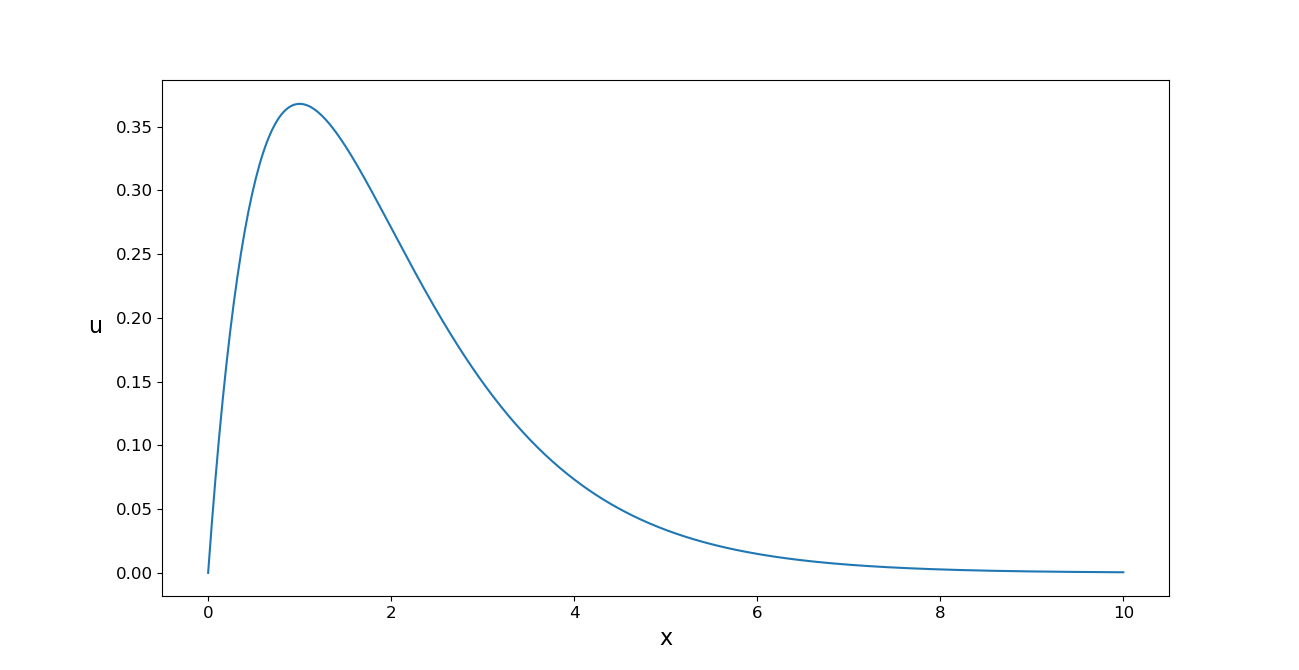
\includegraphics[trim={2.1cm, 0.6cm, 0, 1.5cm}, clip, scale=0.615]{1_psi.png}
	\caption{Заданная функция $\psi(x)$}
	\label{fig:image1}
\end{figure}

\begin{figure}[H]
	\centering
	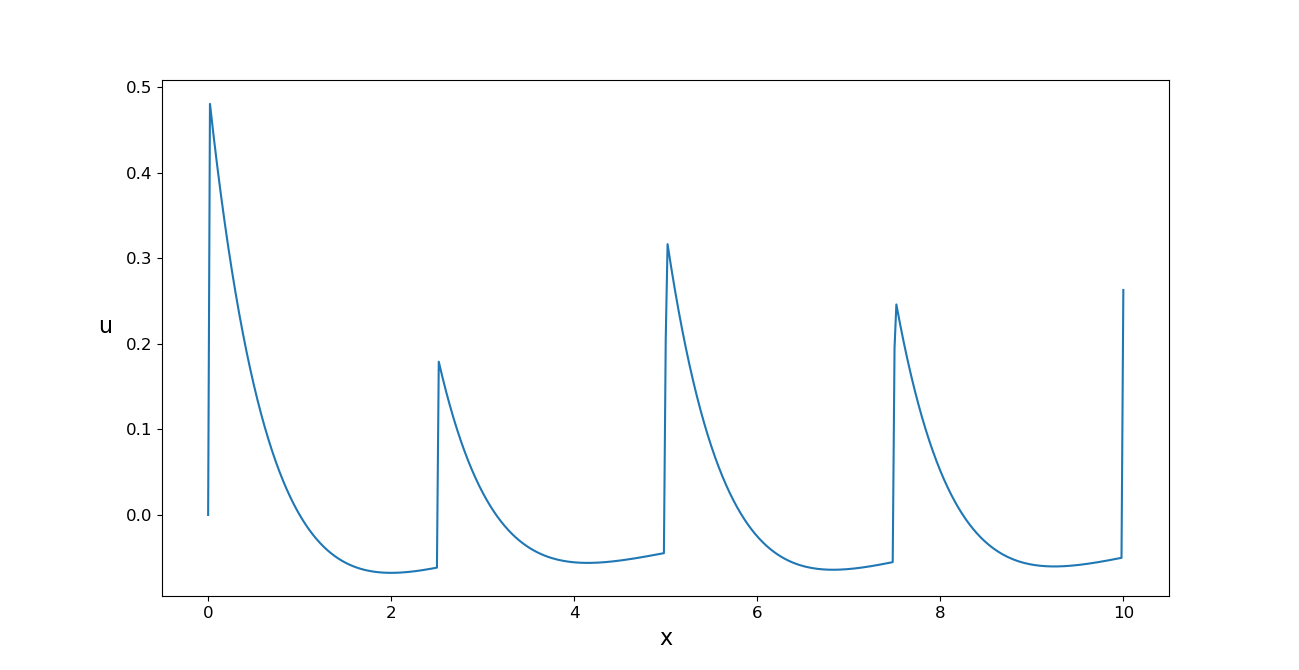
\includegraphics[trim={2.1cm, 0.6cm, 0, 1.5cm}, clip, scale=0.615]{1_u0.png}
	\caption{Найденная функция $\varphi(x)$}
	\label{fig:image2}
\end{figure}

Начальное условие $\varphi(x)$ соответствует обобщённому решению $u(x,t)$ в пространстве $L_1[0,l]$.

\newpage

\subsection{Пример 2}
Входные данные: $\tau_1 = 2.5$, $\;[\alpha_1;\, \alpha_2] = [1;\, 2]$, $\;\psi(x) = x \arctg(x)$.
\begin{figure}[H]
	\centering
	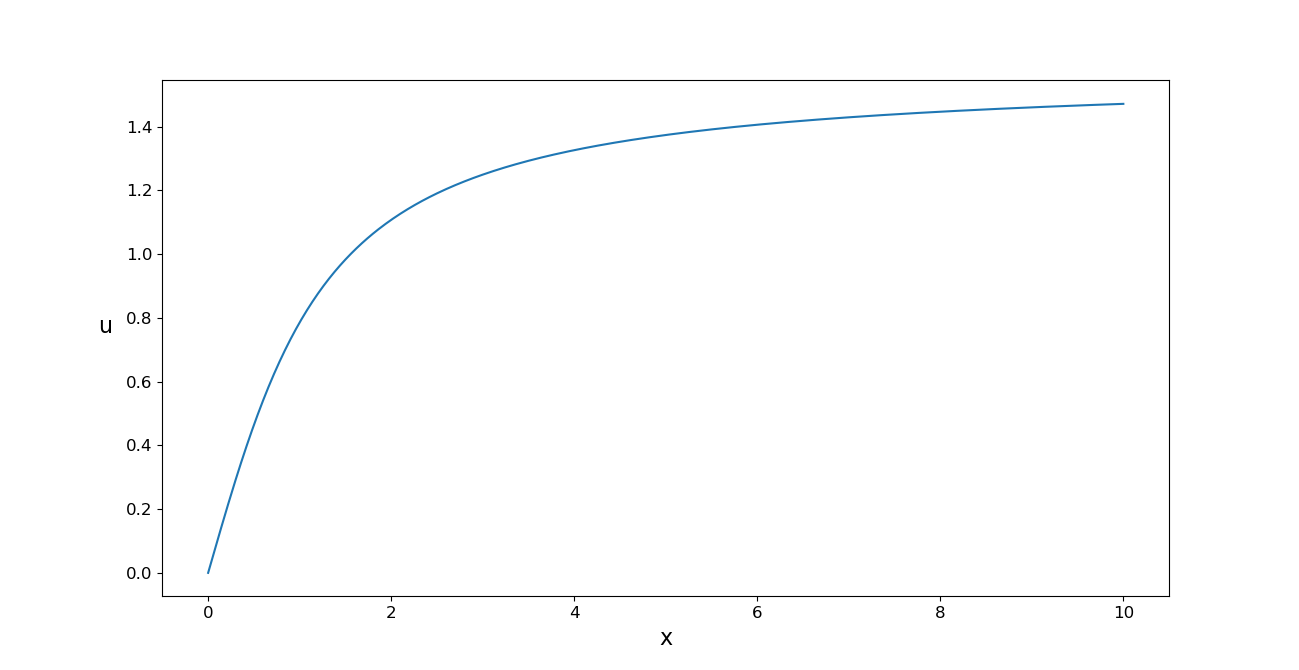
\includegraphics[trim={2.5cm, 0, 0, 1.5cm}, clip, scale=0.62]{2_psi.png}
	\caption{Заданная функция $\psi(x)$}
	\label{fig:image4}
\end{figure}

\begin{figure}[H]
	\centering
	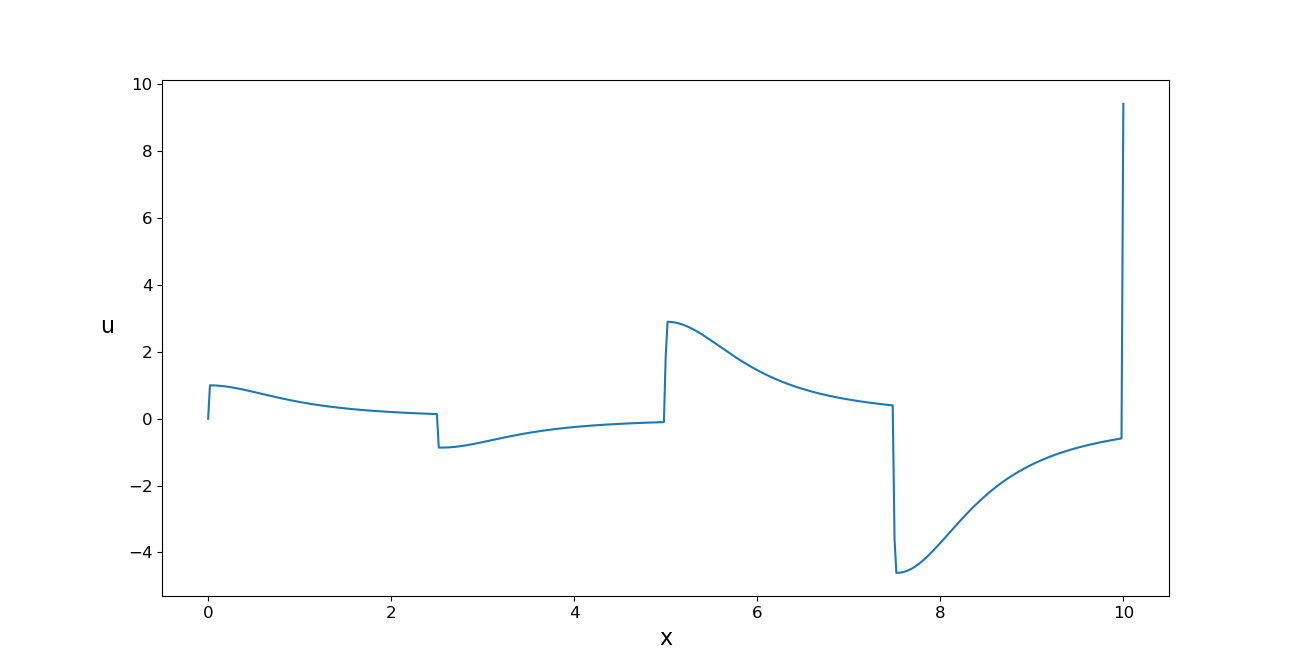
\includegraphics[trim={2.5cm, 0, 0, 1.5cm}, clip, scale=0.62]{2_u0.png}
	\caption{Найденная функция $\varphi(x)$}
	\label{fig:image5}
\end{figure}

Начальное условие $\varphi(x)$ соответствует обобщённому решению $u(x,t)$ в пространстве $L_1[0,l]$. При этом
$\varphi(x) \in C[0,l]$.

\newpage

\subsection{Пример 3}
Входные данные: 
$\tau_1 = 2.5$, $\;[\alpha_1;\, \alpha_2] = [1;\, 2]$, $\;\psi(x) = x^3(10 - x)$.
\begin{figure}[H]
	\centering
	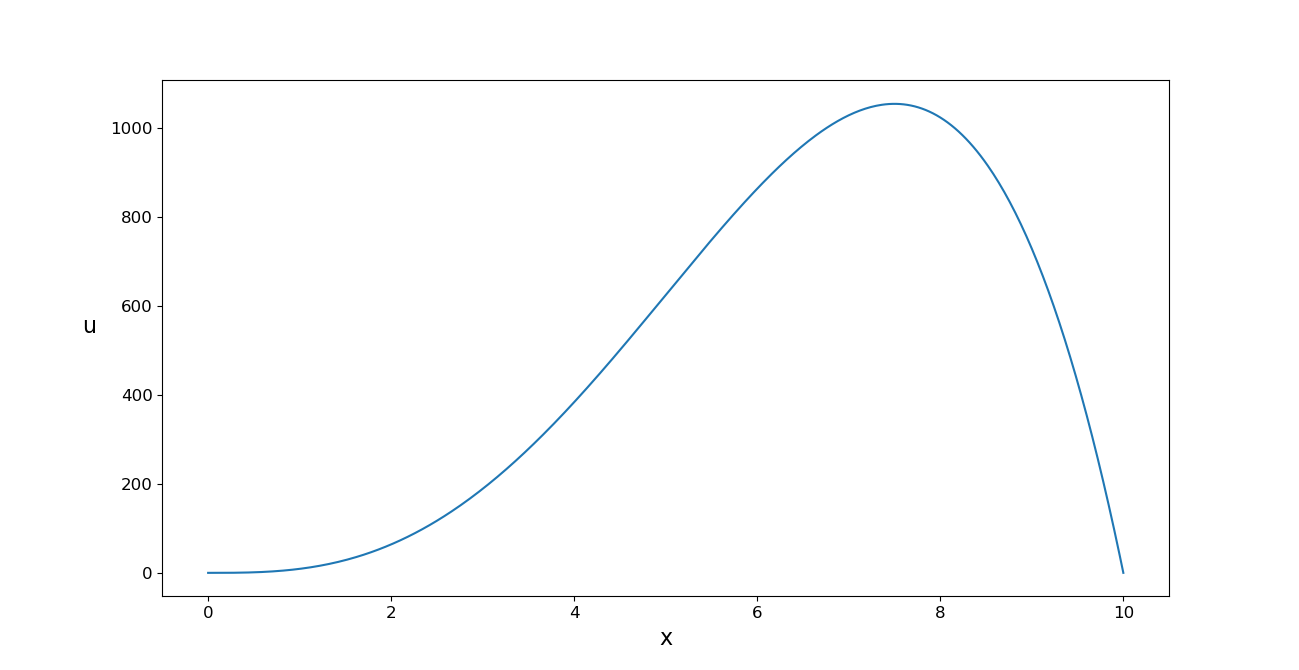
\includegraphics[trim={2.02cm, 0, 0, 1.5cm}, clip, scale=0.61]{3_psi.png}
	\caption{Найденная функция $\psi(x)$}
	\label{fig:image7}
\end{figure}
\begin{figure}[H]
	\centering
	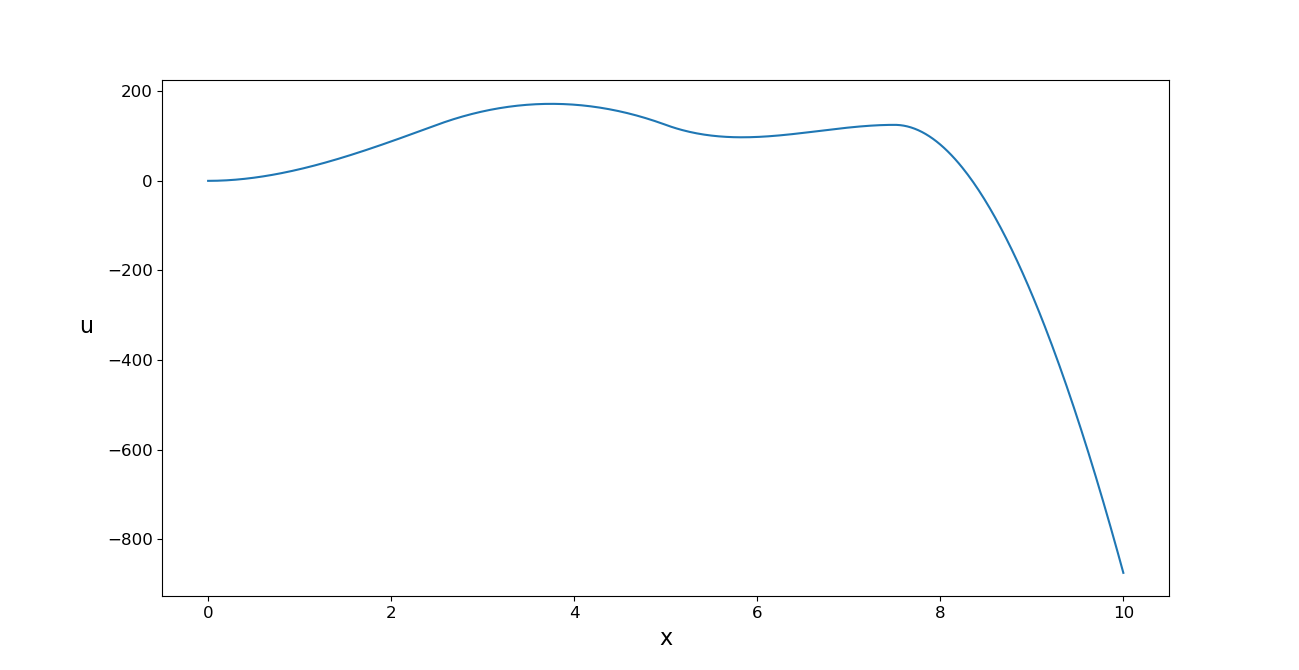
\includegraphics[trim={2.02cm, 0, 0, 1.5cm}, clip, scale=0.61]{3_u0.png}
	\caption{Найденная функция $\varphi(x)$}
	\label{fig:image8}
\end{figure}

Начальное условие соответсвует классическому решению $u(x,t)$ в пространстве $L_1[0,l]$. При этом
$\varphi(x) \in C^2[0,l]$.

\newpage

\subsection{Пример 4}
Входные данные: \\
$[\tau_1;\, \tau_2] = [1.666;\, 3.333]$, $\;[\alpha_1;\, \alpha_2;\, \alpha_3] = [3;\, 2;\, 1]$, 
$\;\psi(x) = x - \sin(x)$.
\begin{figure}[H]
	\centering
	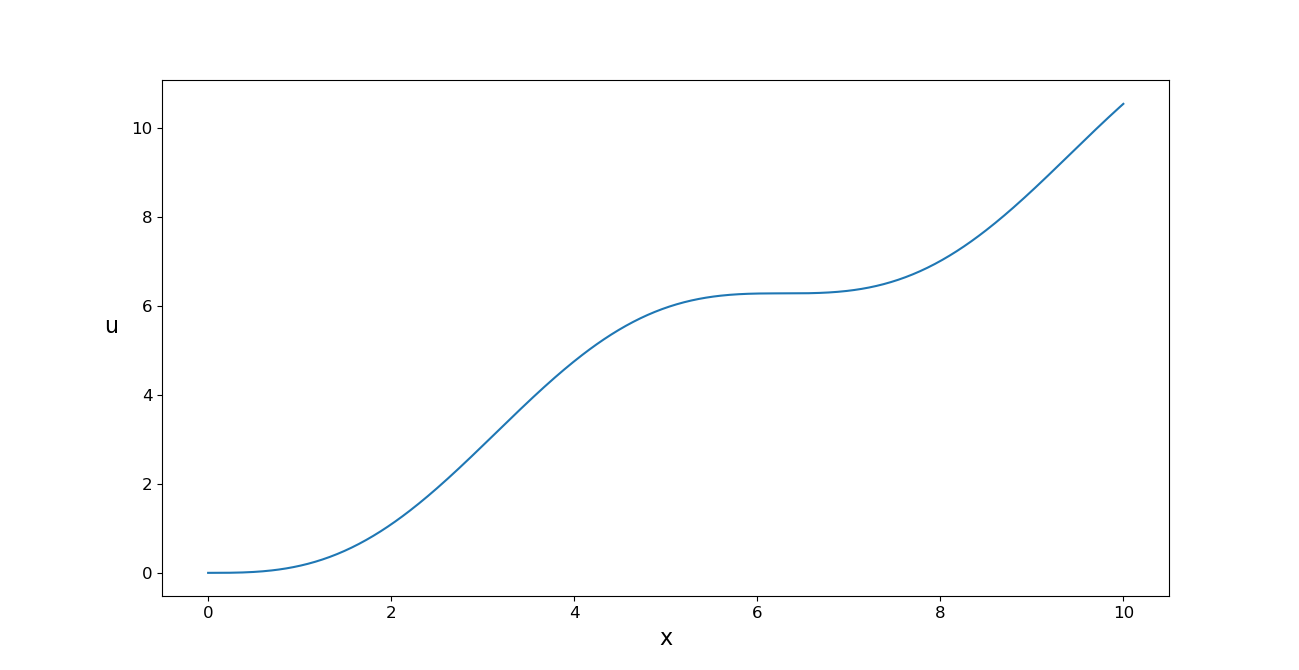
\includegraphics[trim={2.475cm, 0, 0, 1.5cm}, clip, scale=0.624]{410_psi.png}
	\caption{Заданная функция $\psi(x)$}
	\label{fig:image9}
\end{figure}

\begin{figure}[H]
	\centering
	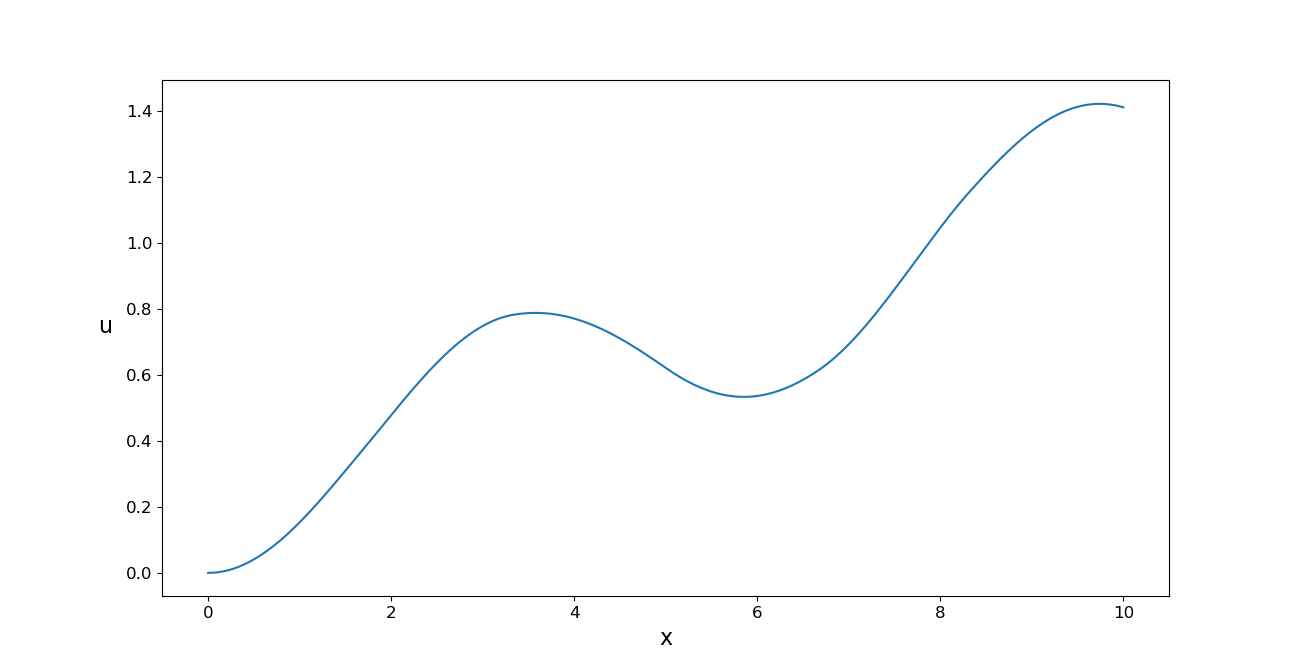
\includegraphics[trim={2.3cm, 0, 0, 1.5cm}, clip, scale=0.62]{4_u0.png}
	\caption{Найденная функция $\varphi(x)$}
	\label{fig:image10}
\end{figure}

\newpage
\subsection{Пример 5}
Входные данные: \\
$[\tau_1;\, \tau_2] = [1.666;\, 3.333]$, $\;[\alpha_1;\, \alpha_2;\, \alpha_3] = [1;\, 2;\, 3]$, 
$\;\psi(x) = x - \sin(x)$.
\begin{figure}[H]
	\centering
	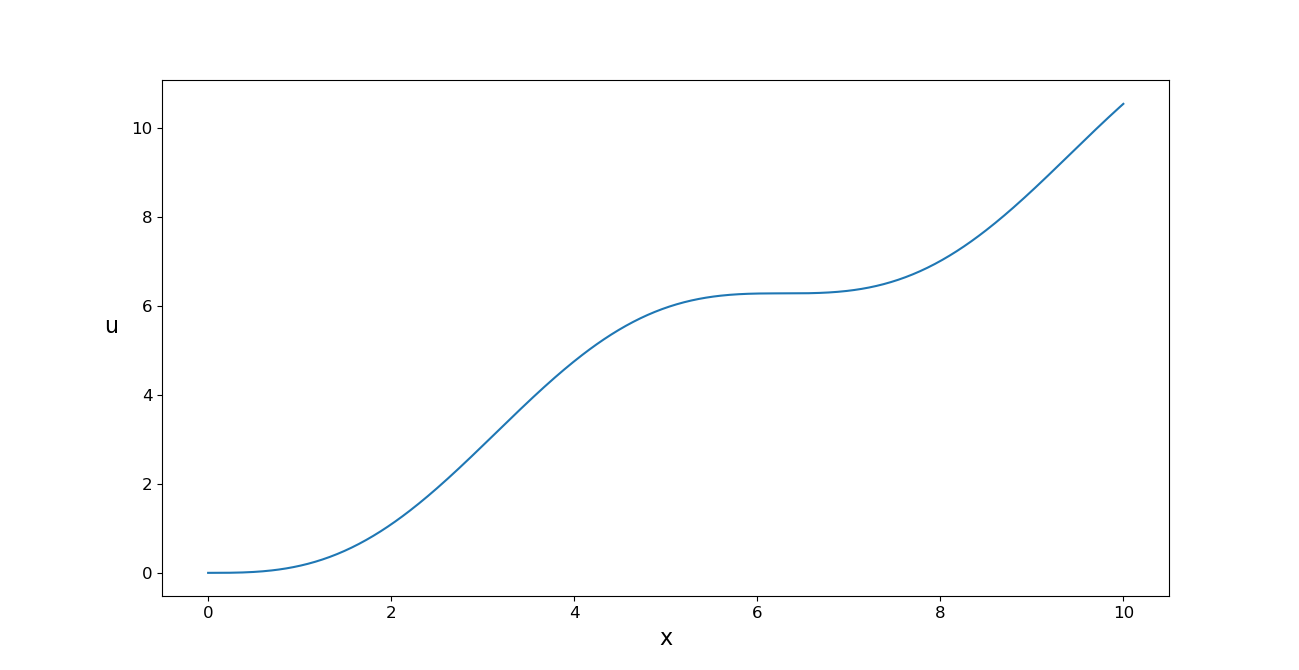
\includegraphics[trim={2.475cm, 0, 0, 1.5cm}, clip, scale=0.624]{410_psi.png}
	\caption{Заданная функция $\psi(x)$}
	\label{fig:image90}
\end{figure}

\begin{figure}[H]
	\centering
	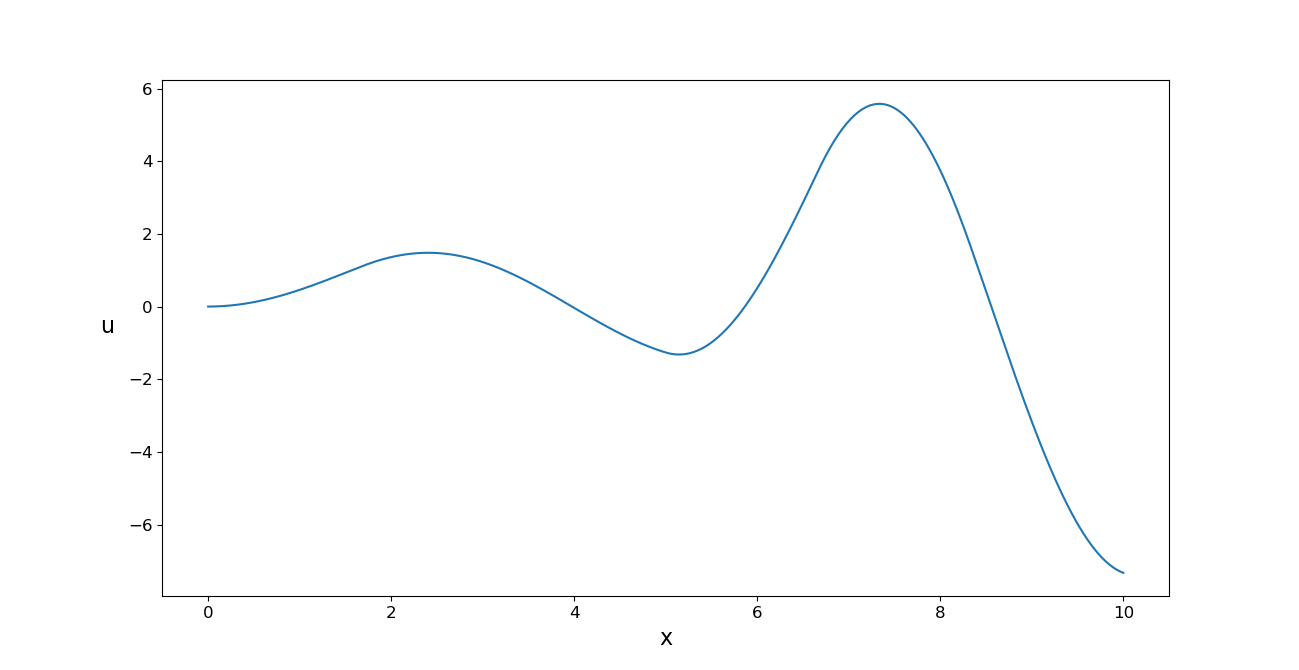
\includegraphics[trim={2.3cm, 0, 0, 1.5cm}, clip, scale=0.62]{10_u0.png}
	\caption{Найденная функция $\varphi(x)$}
	\label{fig:image130}
\end{figure}

\newpage

\subsection{Пример 6}
Входные данные: 
$[\tau_1;\, \tau_2;\, \tau_3;\, \tau_4] = [1;\, 2;\, 3;\, 4]$, \\[1mm]
$[\alpha_1;\, \alpha_2;\, \alpha_3;\, \alpha_4;\, \alpha_5] = [2;\, 1;\, 2;\, 1;\, 2]$, 
$\,\psi(x) = \arctan(x)(1 - \cos(x))$.
\begin{figure}[H]
	\centering
	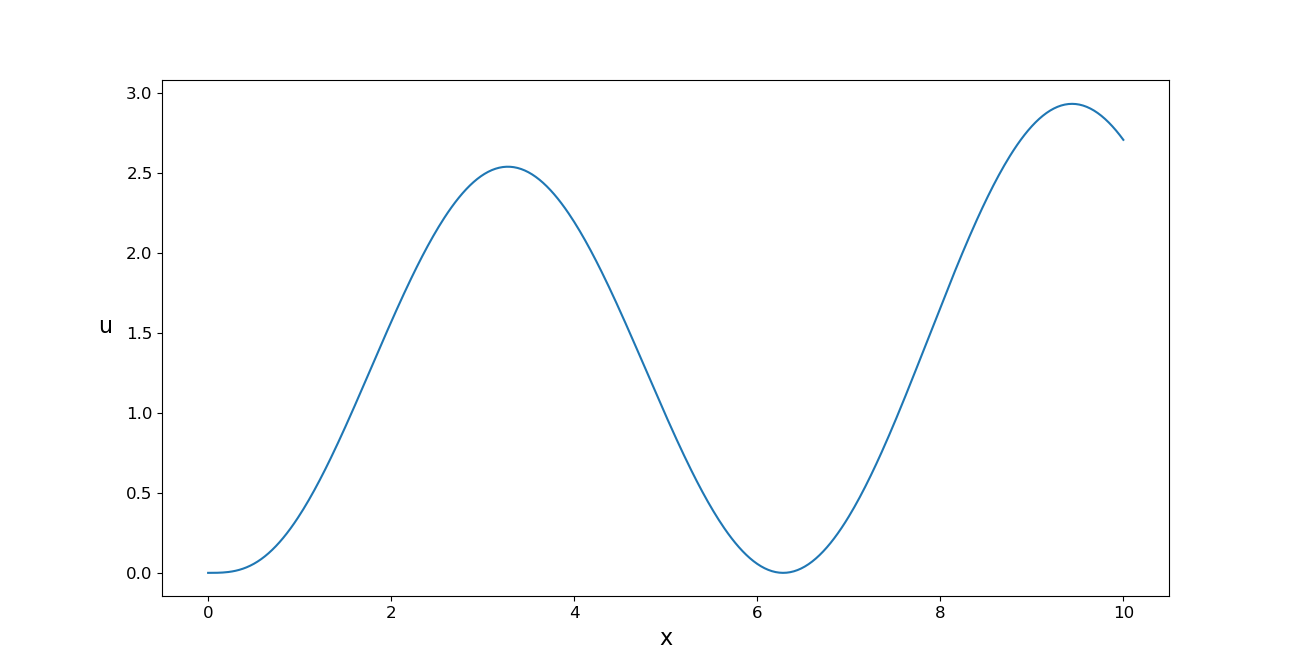
\includegraphics[trim={2.475cm, 0, 0, 1.5cm}, clip, scale=0.624]{56_psi.png}
	\caption{Заданная функция $\psi(x)$}
	\label{fig:image13}
\end{figure}

\begin{figure}[H]
	\centering
	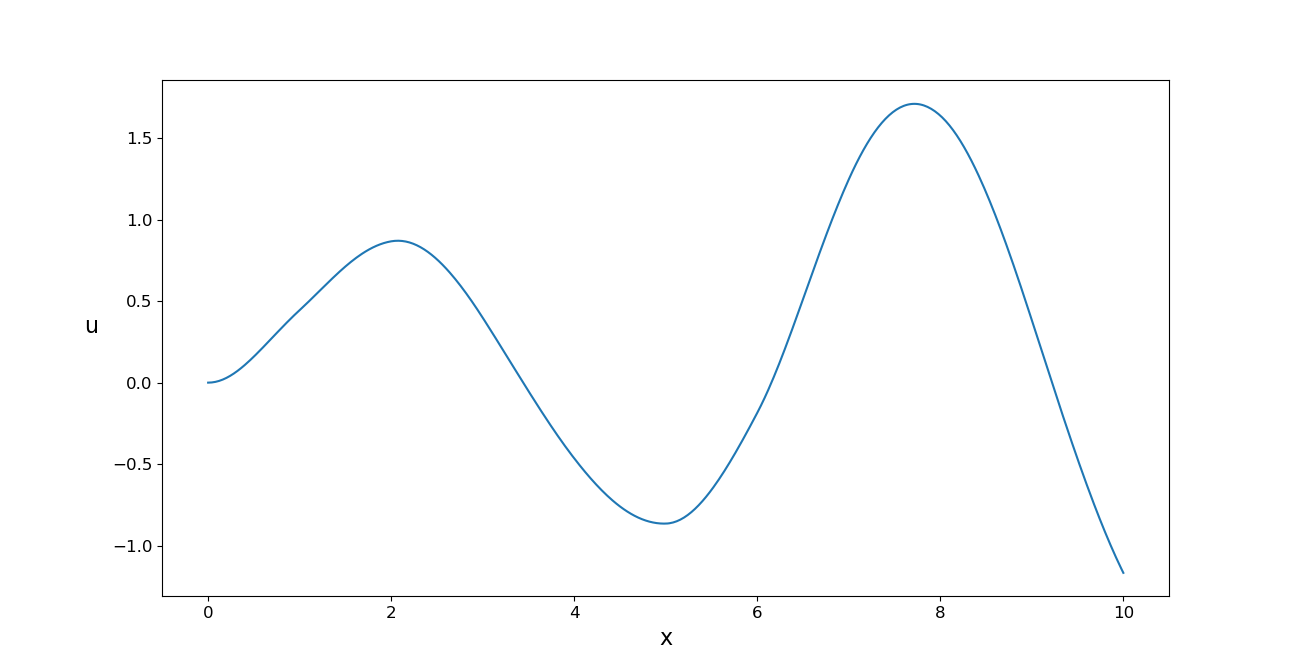
\includegraphics[trim={2.15cm, 0, 0, 1.5cm}, clip, scale=0.618]{5_u0.png}
	\caption{Найденная функция $\varphi(x)$}
	\label{fig:image14}
\end{figure}

\newpage

\subsection{Пример 7}
Входные данные: 
$[\tau_1;\, \tau_2;\, \tau_3;\, \tau_4] = [1;\, 2;\, 3;\, 4]$, \\[1mm]
$[\alpha_1;\, \alpha_2;\, \alpha_3;\, \alpha_4;\, \alpha_5] = [1;\, 2;\, 1;\, 2;\, 1]$, 
$\;\psi(x) = \arctan(x)(1 - \cos(x))$.
\begin{figure}[H]
	\centering
	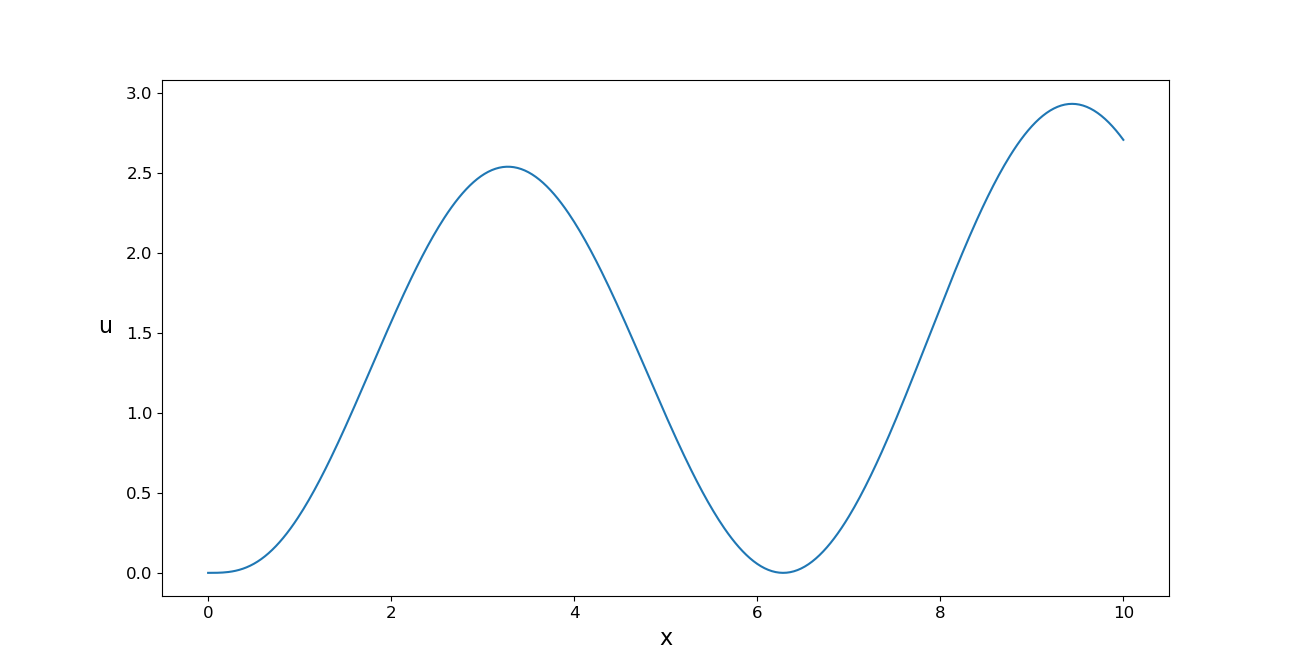
\includegraphics[trim={2.475cm, 0, 0, 1.5cm}, clip, scale=0.624]{56_psi.png}
	\caption{Заданная функция $\psi(x)$}
	\label{fig:image11}
\end{figure}

\begin{figure}[H]
	\centering
	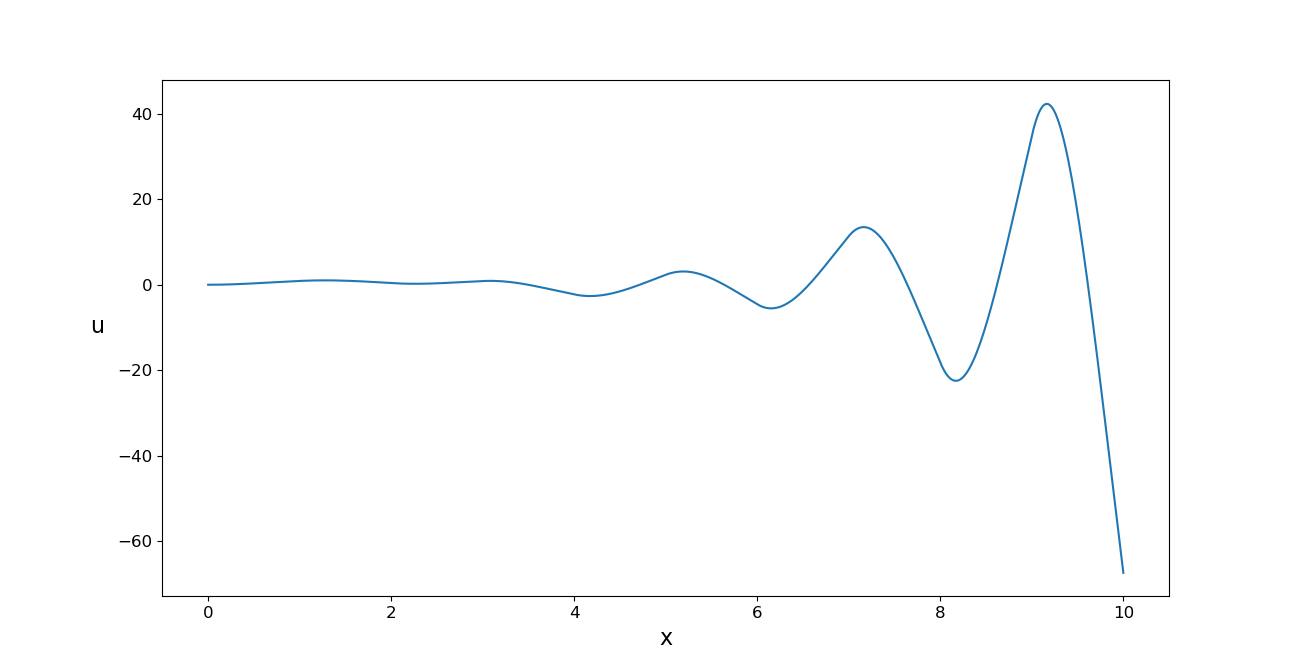
\includegraphics[trim={2.175cm, 0, 0, 1.5cm}, clip, scale=0.618]{6_u0.png}
	\caption{Найденная функция $\varphi(x)$}
	\label{fig:image12}
\end{figure}

\newpage

\subsection{Пример 8}
Входные данные: \\
$[\tau_1;\, \tau_2] = [1.666;\, 3.333]$, 
$\;[\alpha_1;\, \alpha_2;\, \alpha_3] = [1;\, 2;\, 3]$,
$\;\psi(x) = x^3$.
\begin{figure}[H]
	\centering
	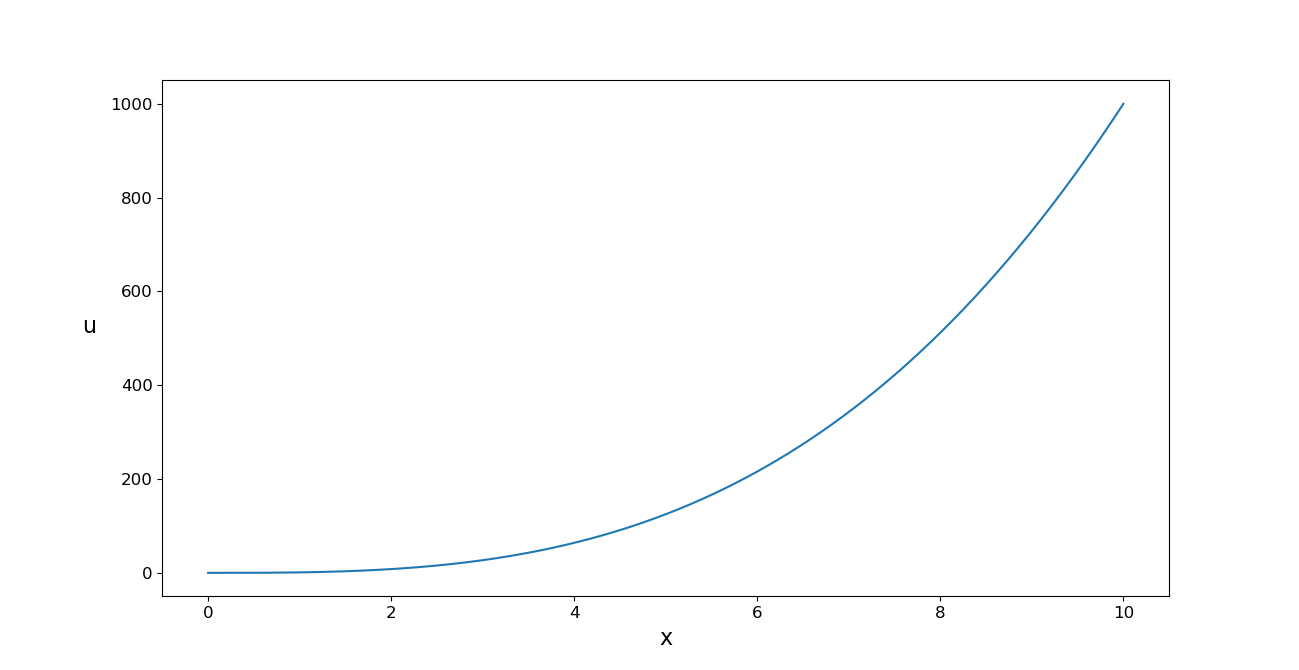
\includegraphics[trim={2.475cm, 0, 0, 1.5cm}, clip, scale=0.624]{789_psi.png}
	\caption{Заданная функция $\psi(x)$}
	\label{fig:image15}
\end{figure}

\begin{figure}[H]
	\centering
	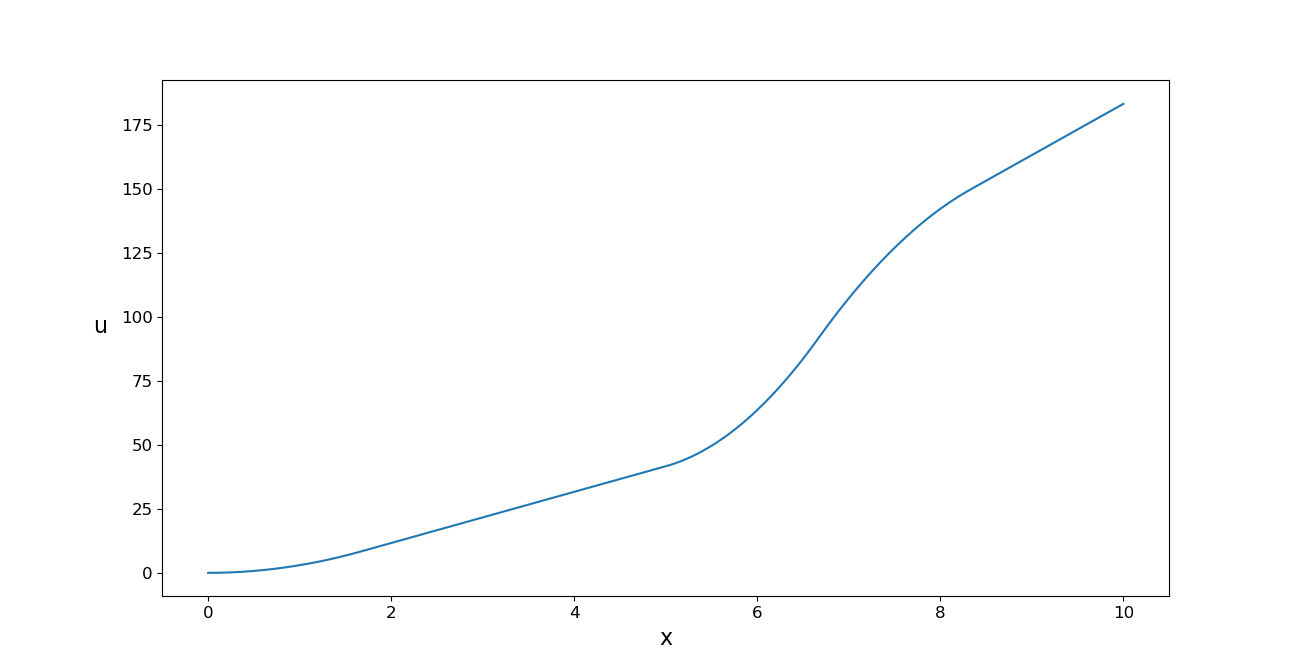
\includegraphics[trim={2.175cm, 0, 0, 1.5cm}, clip, scale=0.618]{7_u0.png}
	\caption{Найденная функция $\varphi(x)$}
	\label{fig:image16}
\end{figure}

\newpage

\subsection{Пример 9}
Входные данные: \\
$[\tau_1;\, \tau_2;\, \tau_3;\, \tau_4] = [1;\, 2;\, 3;\, 4]$, 
$[\alpha_1;\, \alpha_2;\, \alpha_3;\, \alpha_4;\, \alpha_5] = [1;\, 2;\, 3;\, 4;\, 5]$, 
$\,\psi(x) = x^3$.
\begin{figure}[H]
	\centering
	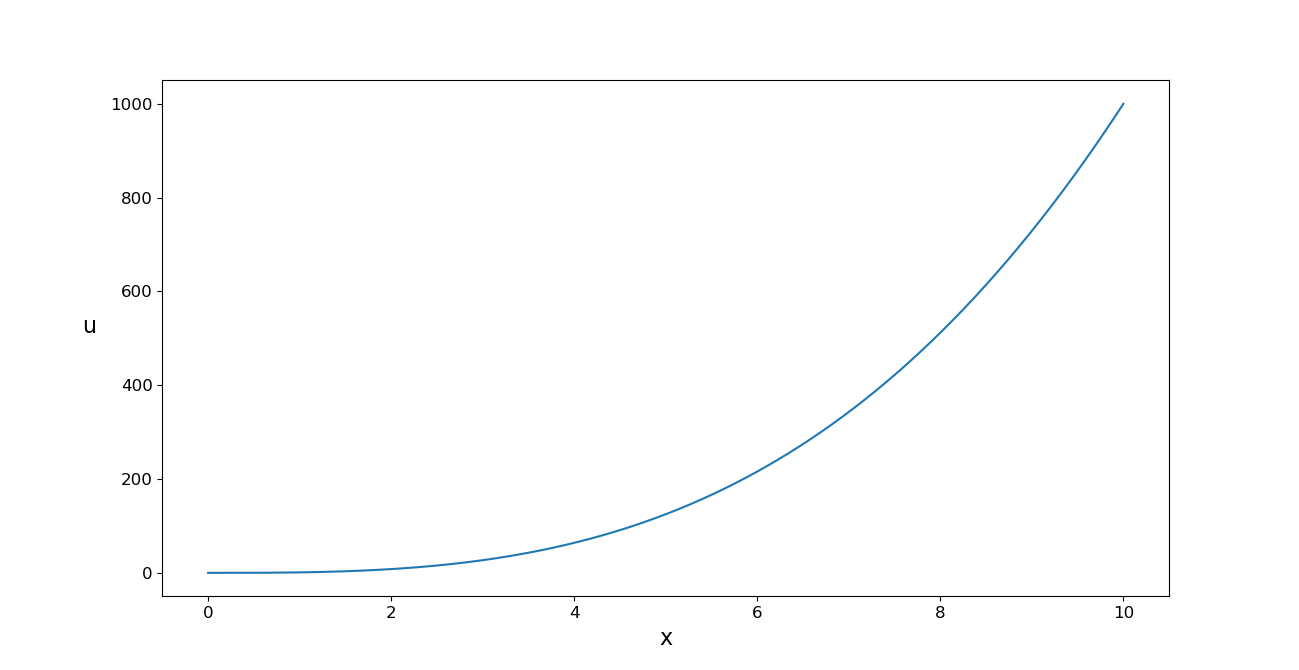
\includegraphics[trim={2.475cm, 0, 0, 1.5cm}, clip, scale=0.624]{789_psi.png}
	\caption{Заданная функция $\psi(x)$}
	\label{fig:image17}
\end{figure}

\begin{figure}[H]
	\centering
	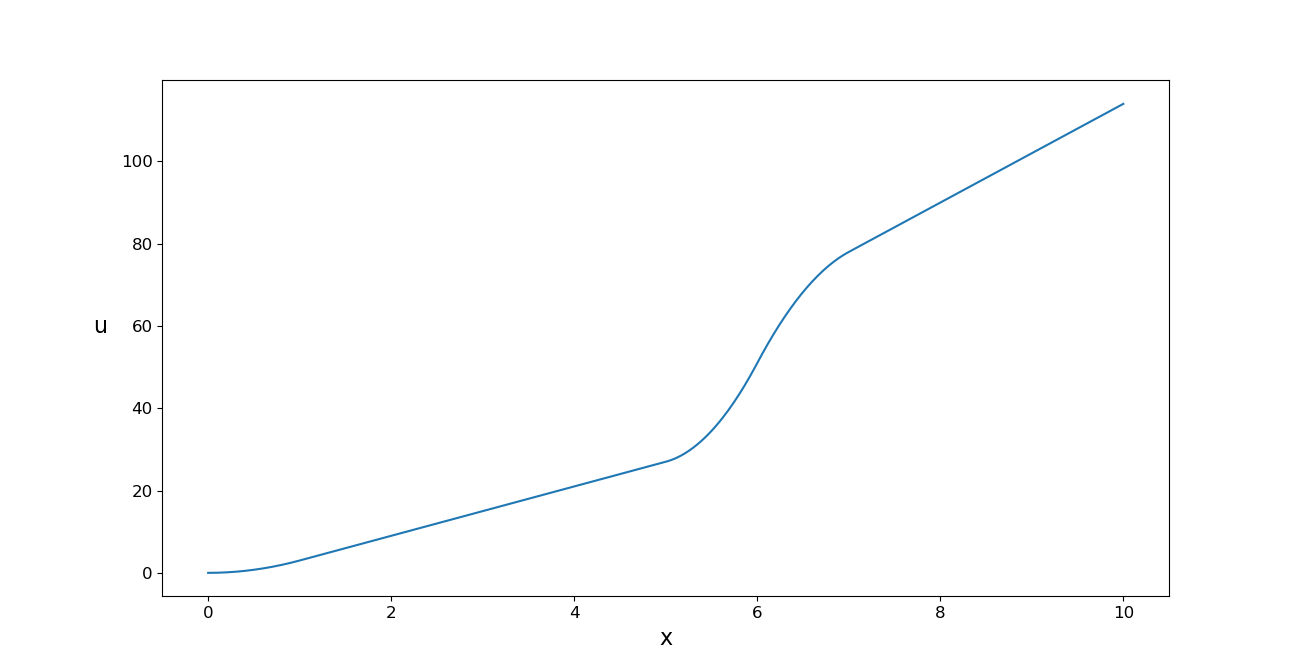
\includegraphics[trim={2.175cm, 0, 0, 1.5cm}, clip, scale=0.618]{8_u0.png}
	\caption{Найденная функция $\varphi(x)$}
	\label{fig:image18}
\end{figure}

\newpage

\subsection{Пример 10}
Входные данные: \\
$[\tau_1;\, \tau_2;\, \tau_3;\, \tau_4;\, \tau_5;\, \tau_6;\, \tau_7] = 
[0.625;\, 1.25;\, 1.875;\, 2.5;\, 3.125;\, 3.75;\, 4.375]$, \\[1mm]
$[\alpha_1;\, \alpha_2;\, \alpha_3;\, \alpha_4;\, \alpha_5;\, \alpha_6;\, \alpha_7;\, \alpha_8] = 
[1;\, 2;\, 3;\, 4;\, 5;\, 6;\, 7;\, 8]$, 
$\,\psi(x) = x^3$.
\begin{figure}[H]
	\centering
	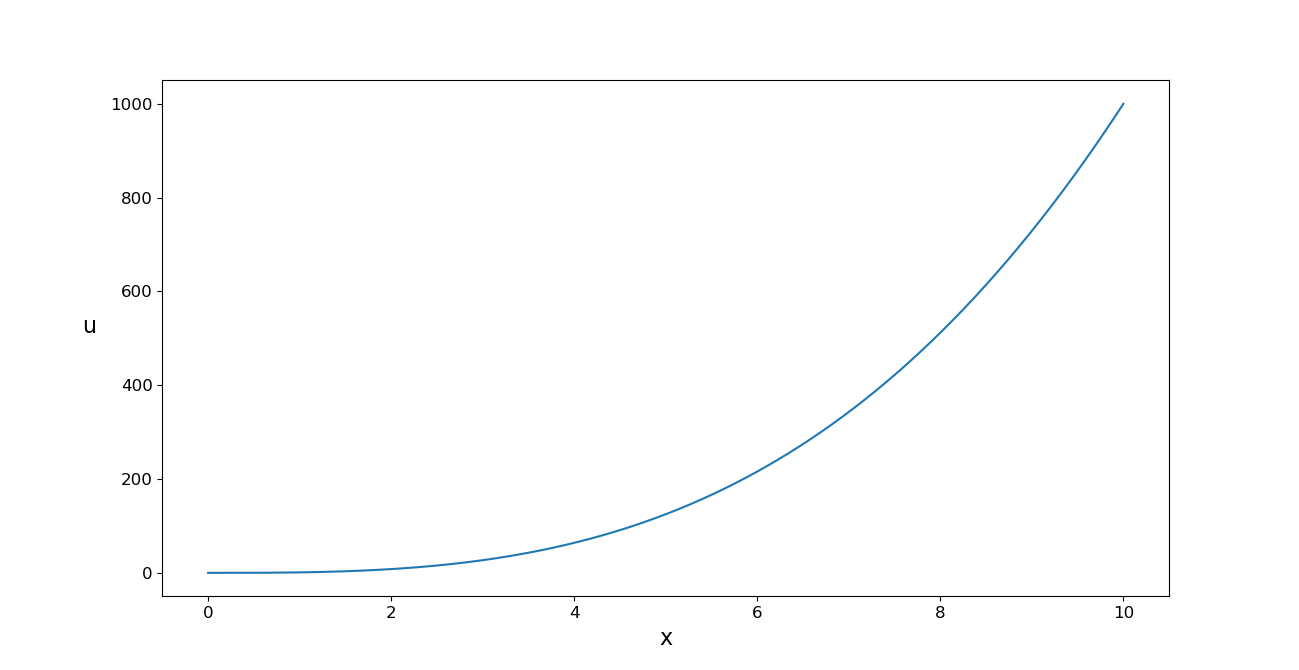
\includegraphics[trim={2.475cm, 0, 0, 1.5cm}, clip, scale=0.624]{789_psi.png}
	\caption{Заданная функция $\psi(x)$}
	\label{fig:image19}
\end{figure}

\begin{figure}[H]
	\centering
	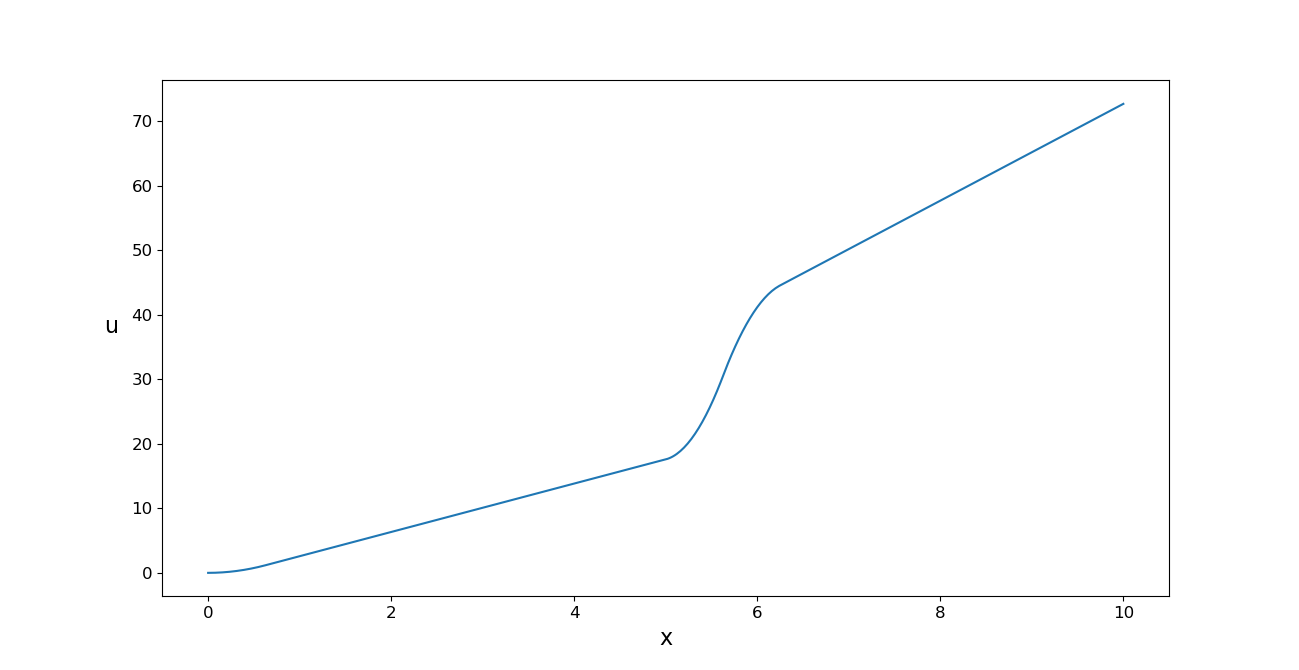
\includegraphics[trim={2.175cm, 0, 0, 1.5cm}, clip, scale=0.618]{9_u0.png}
	\caption{Найденная функция $\varphi(x)$}
	\label{fig:image20}
\end{figure}

\newpage

\section*{Заключение}
\addcontentsline{toc}{section}{Заключение}
В настоящей работе рассмотрен вопрос о конструктивном нахождении решения нело-
кальной по времени задачи для одномерного уравнения теплопроводности, при этом:
\begin{enumerate}
	\item Проведён подробный вывод решения абстрактной нелокальной задачи, установлены условия существования и единственности её решения.
	
	\item Формула решения абстрактной нелокальной задачи перенесена на случай исходной нелокальной задачи.
	
	\item Составлен алгоритм решения поставленной нелокальной задачи.
	
	\item Разработана компьютерная программа, которая реализует алгоритм решения и визуализурует результаты вычислений.
	
	\item Проведена большая серия вычислительных экспериментов, подтвердившая высокую надежность алгоритма.
\end{enumerate}
В результате проделанной работы все поставленные цели достигнуты и исследование
можно считать завершенным.
\newpage

\begin{thebibliography}{99}
	
\addcontentsline{toc}{section}{\bibname}

	\bibitem{Tikhonov1} Тихонов~И.~В., Ву~Нгуен~Шон~Тунг.
	\emph{Разрешимость нелокальной задачи для эволюционного уравнения с суперустойчивой полугруппой}
	// Дифференциальные уравнения. 2020. Т. 56. №4. С. 490-510.
	
	\bibitem{Tikhonov2} Тихонов~И.~В., Ву~Нгуен~Шон~Тунг.
	\emph{Формулы явного решения в модельной нелокальной задаче для уравнения простого переноса}
	// Математические заметки СВФУ. 2017. Т. 24. № 1. С. 57-73.
	
	\bibitem{Balakrishnan_1} Balakrishnan~A.~V.
	\emph{On superstability of semigroups}
	// In: M.P. Polis et al (eds.). Systems modelling and optimization. 
	Proceedings of the 18th IFIP conference on system modelling and optimization. 
	CRC research notes in mathematics. Chapman and Hall. 1999. P. 12–19.
	
	\bibitem{Balakrishnan_2} Balakrishnan~A.~V.
	\emph{Smart structures and super stability} 
	// In: G. Lumer, L. Weis (eds.). Evolution
	equations and their applications in physical and life sciences. Lecture notes in pure and applied
	mathematics. Marcel Dekker. 2001. V. 215. P. 43–53.
	
	\bibitem{Dunford_Schwartz} Данфорд~Н., Шварц~Д.
	\emph{Линейные операторы.} М., 1962, Т.1. Общая теория.
	
	\bibitem{Hille_Phillips} Хилле~Э., Филлипс~Р.
	\emph{Функциональный анализ и полугруппы.} М., 1962.

	\bibitem{Pazy} Pazy~A.
	\emph{Semigroups of linear operators and applications to partial differential equations.} N.Y.: Springer Verlag, 1983.
	
	\bibitem{Kolmogorov_Fomin} Колмогоров~А.~Н., Фомин~С.~В.
	\emph{Элементы теории функций и функционального анализа.} М.: Наука, 1976.
	
	\bibitem{Trenogin} Треногин~В.~А.
	\emph{Функциональный анализ.} 4-е изд. М.: ФИЗМАТЛИТ, 2007.
	
	\bibitem{Filippov} Филиппов~А.~Ф.
	\emph{Введение в теорию дифференциальных уравнений.} М.: Едиториал УРСС, 2004.
\end{thebibliography}

\end{document}
